%\documentclass[12pt,a4paper]{styles}
\documentclass[12pt,a4paper]{report}
%% idioma i codificació 
\usepackage[T1]{fontenc}
\usepackage[utf8]{inputenc}
\usepackage[catalan]{babel}
\usepackage{siunitx}
%%% format de pàgines
\usepackage{geometry}
 \geometry{
 a4paper,
 total={170mm,257mm},
 left=20mm,
 top=20mm,
 }

%%% incloure gràfics
\usepackage{graphicx}

%%% embolicar figura amb text
\usepackage{wrapfig}

%%% font per a fórmules matemàtiques
\usepackage{amsmath,amsthm,amsfonts}
\usepackage{amssymb}
%%% taules llargues
\usepackage{multirow,longtable}

%%% Vertical alignment of a text in a table with figures
\usepackage[export]{adjustbox}

%%% colors
\usepackage{xcolor}
%%\usepackage{blindtext}

%%% line spacing
\usepackage{setspace}
%\spacing{1.213}
%\spacing{1.5}
%\onehalfspacing

%% links 
\usepackage{xurl}
\usepackage{hyperref}
\hypersetup{
    colorlinks=true,
    linkcolor=black,
    filecolor=red, 
    citecolor=red,     
    urlcolor=blue   
    }

%%% format codi python
\usepackage{color}
\definecolor{darkred}{rgb}{0.6,0.0,0.0}
\definecolor{darkgreen}{rgb}{0,0.50,0}
\definecolor{lightblue}{rgb}{0.0,0.42,0.91}
\definecolor{orange}{rgb}{0.99,0.48,0.13}
\definecolor{grass}{rgb}{0.18,0.80,0.18}
\definecolor{pink}{rgb}{0.97,0.15,0.45}

\definecolor{mygreen}{rgb}{0,0.6,0}
\definecolor{mygray}{rgb}{0.5,0.5,0.5}
\definecolor{mymauve}{rgb}{0.58,0,0.82}

\usepackage{listingsutf8}
\usepackage{listings}

\lstset{
  aboveskip=15px,
  language=Python,
  basicstyle=\footnotesize, 
  backgroundcolor=\color{white},
  commentstyle=\color{mygreen},
  frame=single,
  keywordstyle=true,
  keywordstyle=\color{blue},
  breaklines=true,
  postbreak=\mbox{\textcolor{red}{$\hookrightarrow$}\space},
  inputencoding=utf8/latin1,
  literate=
  {á}{{\'a}}1
  {à}{{\`a}}1
  {ã}{{\~a}}1
  {é}{{\'e}}1
  {ê}{{\^e}}1
  {í}{{\'i}}1
  {ó}{{\'o}}1
  {ò}{{\`o}}1
  {õ}{{\~o}}1
  {ú}{{\'u}}1
  {ü}{{\"u}}1
  {ç}{{\c{c}}}1
}

%%% format de taules
\usepackage{booktabs}
\usepackage{tabu}

%%% font helvètica
\usepackage[scaled=1]{helvet}
\renewcommand\familydefault{\sfdefault} 
\renewcommand{\baselinestretch}{1.5}
%\usepackage[helvet]{sfmath}
%\everymath{\rm}

%%% eliminar espai al començament dels paràgrafs
\setlength{\parindent}{0cm}

%%% personalitzar format dels capítols i seccions
\usepackage{titlesec}
%\titleformat{\chapter}[hang]{\normalfont\huge\bfseries}{\chaptertitlename\ \thechapter.}{0.25em}{}
\titleformat{\chapter}[hang]{\normalfont\huge\bfseries\raggedright}{\thechapter.}{0.25em}{}
%\titleformat{\chapter}[hang]{\normalfont\huge\bfseries\raggedright}{\chaptertitlename\ \thechapter.}{0.25em}{}
%\let\chaptername\relax
%\renewcommand{\chaptername}{}
%\renewcommand{\thechapter}{}

\titlespacing{\chapter}{0pt}{-40pt}{20pt}

%%% mida de font de les figures
\usepackage[font=small,labelfont=bf]{caption}


%%\titlespacing{\section}
%%  {0pt}
%%  {-10pt}
%%  {-10pt}  
%\titleformat{\chapter}[hang] 
%{\normalfont\huge\bfseries}{\chaptertitlename\ \thechapter:}{.25em}{}
%

%%% marge entre paràgrafs
\setlength{\parskip}{12pt}

%%% mida itemize
\usepackage{enumitem}
\setlist[itemize]{noitemsep, topsep=0pt}

%% crear bibliografia
%\usepackage[
%backend=biber,
%style=numeric,
%sorting=none
%]{biblatex}
%\usepackage{csquotes}
\usepackage[defernumbers=true, sortcites=true, citestyle=numeric-comp]{biblatex}
\addbibresource{refs.bib}
%\bibliography{refs}



%\usepackage{breakurl}

%\newtheorem{defi}{Definición}[chapter]
%\newtheorem{col}{Corolario}[chapter]
%\newtheorem{teo}{Teorema}[chapter]
%\newtheorem{lem}{Lema}[chapter]
%\newtheorem{pro}{Proposición}[chapter]
%\newtheorem{obs}{Observación}[chapter]
%\newtheorem{eje}{Exemple}[chapter]
%\newtheorem{ejer}{Ejercicio}[chapter]
%\newtheorem{expe}{Experimento}[chapter]
\newtheorem{eje}{Exemple}[chapter]
\newcommand*{\myproofname}{\textbf{Solució}}
\newenvironment{myproof}[1][\myproofname]{\begin{proof}[#1]\renewcommand*{\qedsymbol}{\(\blacksquare\)}}{\end{proof}}

\begin{document}
\tableofcontents\hspace{0cm}
\newpage
\begin{flushright}
\textit{Abans de començar amb el treball en si, donar agraïments a les persones que m'han ajudat a realitzar el TR. Primerament, al meu tutor de TR, per ajudar-me a plantejar el tema i donar-me algunes indicacions de com seguir. També, agrair al meu pare per ajudar-me a entendre i estudiar els conceptes matemàtics que es veuran en el treball.}
\end{flushright}

\chapter*{RESUM}
\addcontentsline{toc}{chapter}{RESUM}
Els fractals representen un gir en el plantejament de la geometria natural. Aquests engloben teories i formes matemàtiques importants avui dia. Eventualment, es va començar a veure la seva viabilitat en aplicacions tecnològiques, formulació de teories i observació de la naturalesa i fenòmens naturals, les quals avui dia es continuen investigant i desenvolupant. En aquest treball es pretén estudiar a fons els fractals i respondre a la següent qüestió: És possible modelar en 3D un paisatge natural a partir d'un sol fractal? Es podran obtenir més d’un tipus de paisatge? Per a dur a terme aquest treball es va fer una recerca a fons sobre el concepte de fractal (característiques, tipus, història, etc.). Aquesta recerca es va realitzar revisant i mirant diferents fonts d'informació (llibres, textos, vídeos i llocs web). Posteriorment, usant programació Python, es va buscar construir diversos models de paisatges ''naturals'', que se semblessin a un paisatge natural real, a partir de seccions d'alguns fractals (conjunt de Mandelbrot, conjunts de Julia i el fractal de Newton). Els resultats obtinguts van ser la generació de diferents models de paisatge ''semblants'' a un model real. Després d'aquests resultats, es demostra que, a través dels conjunts de Mandelbrot, Julia i el fractal de Newton, observem que es poden generar paisatges semblants, a un paisatge natural a partir d'un fragment d'aquest fractal.
\chapter*{ABSTRACT}
Fractals represent a major breakthrough in the approach to natural geometry. They include theories and mathematical forms that are important today. Eventually, their viability began to be seen in technological applications, formulation of theories and observation of nature and natural phenomena, which today continue to be investigated and developed. In this work we intend to study fractals in depth and answer the following questions: Is it possible to model in 3D a natural landscape from a single fractal? Is it possible to obtain more than one type of landscape? In order to carry out this work, a depth research on the concept of fractal (characteristics, types, history, etc.) was done. This research was done by reviewing and looking at different sources of information (books, texts, videos and websites). After that, using Python programming, we built several models of ''natural'' landscapes, resembling a real natural landscape, from sections of some fractals (Mandelbrot set, Julia sets and Newton's fractal). The results obtained were different landscape models ''resembling'' a real model. After these results, it is demonstrated that with the Mandelbrot, Julia and Newton fractal sets, we obtain that landscapes similar to a natural landscape can be generated from a fragment of this fractal.

%Amb això dit, la premissa d'aquest treball és fer un estudi i investigació dels fractals i de tot el que engloben. Aquesta investigació, comprendre primer un estudi del concepte de fractal en la seva totalitat: història,  fonaments matemàtics,  característiques, formes i la seva construcció. També s'observarà l'impacte d'aquestes figueres en el món natural i a la tecnologia. 
\chapter{INTRODUCCIÓ}
El tema d’aquest treball de recerca (TR) se centra en els fractals i en el seu estudi. Les motivacions personals per escollir aquest camp de les matemàtiques com a temàtica del meu TR, va ser la meva fascinació per aquestes formes, les quals havia vist moltes vegades en llibres, vídeos i també a la natura. Això em va enfilar cap a un interès més acadèmic del tema, és a dir, estudiar sobre el concepte de fractal. Els meus objectius teòrics són estudiar les teories matemàtiques involucrades en els fractals. També es busca conèixer quines han sigut les seves repercussions o implicacions teòriques i pràctiques dins de la ciència, més enllà de les matemàtiques. Com a objectius pràctics es busca aprendre a utilitzar un llenguatge de programació (Python), per després elaborar els meus paisatges fractals i respondre a les següents qüestions: És possible modelar en 3D un paisatge natural a partir d'un sol fractal? Es podran obtenir més d’un tipus de paisatge? Amb aquesta premissa, el treball es va orientar inicialment (a part d'en un estudi explicatiu) en un àmbit més tecnològic, sent que es buscava construir una antena amb forma fractal, però, per diverses circumstàncies es va decidir orientar a la seva relació amb els paisatges.

Per desenvolupar aquest treball la metodologia a seguir va ser una primera part recopilatòria d’informació sobre el tema i els temes amb els quals es relaciona transversalment (annexos). Aquesta informació es va obtenir de diverses fonts d’informació: pàgines web de divulgació, vídeos de caràcter divulgatiu, i el més important llibres/textos científics. Per a la part pràctica, s’ha utilitzat programació de codi obert Python i algunes llibreries pròpies per a realitzar-les. En l'àmbit estilístic s’ha utilitzat el programa \LaTeX, orientat en la creació de textos científics. L’estructura del treball s’ha dividit en 7 parts: una primera part on es desglossa l'origen dels fractals, una segona en què es comenta individualment les formes fractals, una tercera on s’exposa les característiques comunes de tota forma fractal, seguit de dues parts, una orientada en la presència dels fractals a la natura i altre a la ciència. Les últimes dues parts se centren en la pràctica i els annexos.


%Els fractals ens han donat l'oportunitat de veure la natura en la seva forma més natural. Des del seu descobriment fa dècades la seva importància ha sigut més rellevant del que es pensava. Ens permet entendre les irregularitats de la natura, una geometria dissenyada únicament pel món que hi havia abans de nosaltres. 
%
%Això és la geometria fractal, la qual ens ha permès explicar matemàticament el comportament de la mateixa natura, respecte a la seva forma. Fenòmens com les formes dels paisatges, els accidents geogràfics i les plantes. També la naturalesa pròpia dels raigs o la formació d’estels a la galàxia. El seu descobriment ha sigut també una font d’innovació en tecnologia i computació. 
%
%Amb aquesta premissa l’objectiu d’aquest treball de recerca és realitzar una investigació dels fractals. Investigar sobre el concepte i tot el que engloba el camp de la geometria fractal (fonaments, característiques, formes i la seva construcció). També, analitzar formacions naturals amb geometria fractal present i indagar en la seva importància en la tecnologia i ciència moderna i analitzar la seva viabilitat futura de cara a la investigació i innovació. Per tant, el que es busca és analitzar a fons el concepte fractal i quin impacte ha tingut en el món, tant a la natura com a la tecnologia moderna.
\chapter{DESGLOSANT ELS FRACTALS}
\section{Definició de fractal}
Si s'ha de definir de manera simple i concreta ''que és una fractal?'' la resposta més senzilla seria la geometria del món. La curiositat per tot el que ens envolta és una característica intrínseca dels éssers humans, la qual està present dins nosaltres des que obtenim consciència a la nostra infantesa. Per fer-ho utilitzem descripcions, que obtenim d'allò que els nostres sentits ens permet veure.

La geometria clàssica euclidiana és suficient per explicar la forma dels elements, ara bé, la cosa es dificulta a l'hora d'afrontar formes més complexes: la silueta dels arbres en hivern, les formes de les ones en trencar-se, la ramificació pulmonar, recorregut de la costa, etc. Què són aquestes formes? Com les classifiquem? La resposta a aquestes preguntes són els fractals, formes geomètriques amb molta complexitat, resultat de la repetició d’una forma geomètrica específica, això, gràcies a una particularitat d'aquestes formes anomenada complexa d’autosimilitud, el qual tot i que es desglossarà més endavant, es pot definir com la propietat d'una forma de mantenir-se semblant o quasi semblant a diferents escales.
\begin{figure}[ht!]
\centering
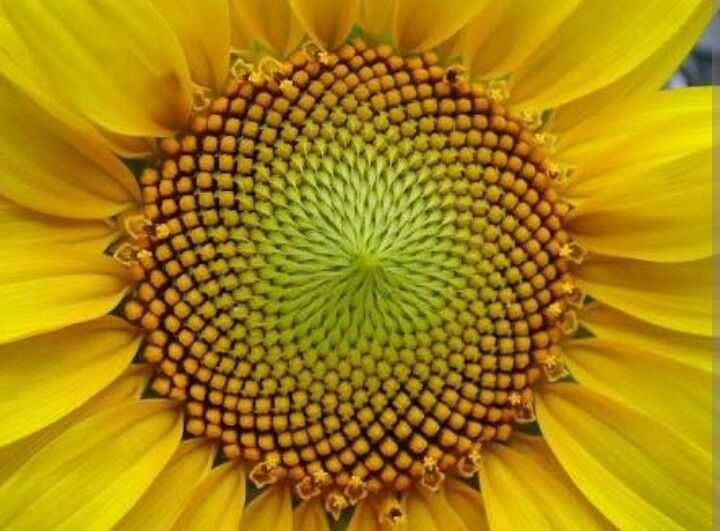
\includegraphics[width=0.6\textwidth]{img/img01_01_girasol}
\caption{Les llavors d'un gira-sol, disposades en dues famílies d'espirals entrellaçades \cite{HistoriaFractales}.}
\label{img01_01}
\end{figure}
\section{Història dels fractals}
Els fractals són el resultat de la necessitat de categoritzar a aquelles formes o figures que la geometria euclidiana no podia definir. Històricament, els humans utilitzàvem la geometria clàssica o euclidiana, descoberta per Euclides fa 2500 anys, per definir a aquelles formes que veiem del nostre voltant. Tot i això, el pas del temps i el desenvolupament de les matemàtiques va necessitar l'aparició d’un nou concepte per aquelles figueres exageradament complexes o ''informes''.

Al segle XIX, la concepció de dimensió que es tenia en aquella època va ser qüestionada pels matemàtics quan investigant aquestes figueres complexes van descobrir que tenien la particularitat de tenir dimensió fraccionària.
\begin{figure}[!ht]
\centering
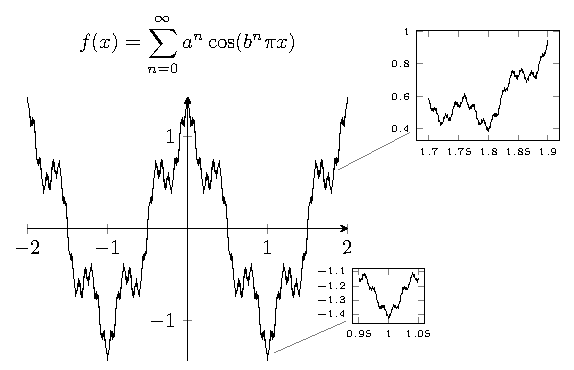
\includegraphics[width=0.65\textwidth]{img/img01_02_weierstrass}
\caption{Representació de la funció de Weierstrass.}
\label{img01_02}
\end{figure}
El principi d’aquest esdeveniment es va donar amb el matemàtic Karl Weierstrass, quan en 1872, va dibuixar la seva funció de Weierstrass (veure Figura \ref{img01_02}). En el mateix segle, van començar a aparèixer conceptes cada vegada més geomètrics i menys algebraics. Aquests conceptes podien construir-se partint d'una figura inicial (iniciador), a la qual s'aplicaven una sèrie de construccions geomètriques senzilles. La sèrie de figures obtingudes s'aproximava a una figura límit que corresponia al que avui diem conjunt fractal. Així, en 1904, Helge Von Koch va definir una corba amb propietats similars a la de Weierstrass: la corba de Koch. En 1915, Waclaw Sierpiński va construir el seu triangle i, un any després, la seva catifa.

Altres dos grans matemàtics que es van endinsar en el camp dels fractals van ser Georg Cantor i Giuseppe Peano. Aquests dos matemàtics van pertànyer a un grup que per la seva labor va ser reconegut cap al final de la ''crisi dels fonaments'' que acabaria en 1925. Un dels problemes tractats durant aquesta crisi dels fonaments va ser que les ''matemàtiques clàssiques'' eren les eines adequades per a estudiar les estructures regulars de la geometria d'Euclides i l'evolució contínua de la dinàmica de Newton, però que eren ineficients amb aquelles formes o estructures que no encaixaven en aquesta mena de geometria.

Sota aquesta premissa es necessitava una ''nova matemàtica'' en la qual encaixessin aquelles formes dissidents amb els patrons de Newton i Euclides, com són la corba de Cantor i la corba de Peano, les quals són capaces "d'omplir el pla". La qüestió sorgeix del següent fet: en ser una corba hauria de tenir dimensió 1, però, si pot emplenar un quadrat la seva dimensió ha de ser 2, per tant, quina és la dimensió d'aquestes estructures? Aquests nous elements no estaven contemplats en la matemàtica tradicional, van ser considerats com a ''monstres matemàtics''.

L'any 1919, Félix Hausdorff va introduir la primera manera d'observar i estudiar aquest tipus de formes en la vida real, la dimensió de Hausdorff-Besicovitch, actualment coneguda com a dimensió fractal. Uns anys més tard, el rus Andrei Kolgomórov descrivia una eina similar a la de Hausdorff que seria posteriorment coneguda com l'entropia de Kolmogórov. Si bé les aportacions d'aquests matemàtics van ser vitals per la formació del que serien els fractals, és al matemàtic Benoît Mandelbrot, a qui hem de mirar com a referent de la geometria fractal.
\section{Benoît Mandelbrot}
\begin{wrapfigure}[9]{l}{0.45\textwidth}
  \begin{center}\vspace{-25pt}
    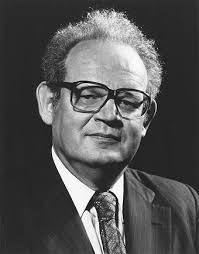
\includegraphics[width=0.3\textwidth]{img/img01_03_mandelbrot.jpeg}
  \end{center}
\end{wrapfigure}
Benoît Mandelbrot \cite{Wikipedia2024:Mandelbrot} va néixer l'any 1924 a Varsòvia, en el si d’una família jueva lituana, en la qual, va tenir als seus dos oncles com a referents, els qui ho van introduir en les matemàtiques. Amb 11 anys, l'any 1936, abandona Polònia a causa de la Segona Guerra Mundial, traslladant-se a França, on la seva educació va caure en mans del seu oncle Szolem Mandelbrot. Aquí comença la trajectòria acadèmica de Mandelbrot, que igual que la seva gran aportació a les matemàtiques, va ser irregular. 

Va realitzar els seus estudis universitaris a la Universitat de Lió, per a després ingressar l’École polytechnique. Temps després, va emigrar cap als Estats Units on va obtenir un màster en aeronàutica a l'Institut Tecnològic de Califòrnia. Va tornar a París per obtenir el doctorat a la Universitat de París l'any 1952. Més endavant va tornar als EUA se'n va anar al MIT i després a l'Institut d'Estudis Avançats de Princeton, on va ser estudiant de John von Neumann. Més endavant va començar a treballar a l'IBM Research.

Paral·lelament, Mandelbrot es va dedicar a investigar sobre aquelles formes que escapaven de la geometria convencional, va examinar els treballs previs de Hausdorff i Gaston Julia, d’aquest últim, va ser alumne i va estudiar molts dels seus articles, els quals no el van interessar en aquell moment. Més endavant, l'any 1967, Mandelbrot va publicar l’article ''Quina longitud té la costa de la Gran Bretanya?'' per a la revista Science. En aquest article, Mandelbrot explicava les seves primeres idees respecte als fractals, que encara el concepte no estava ben definit. En el llibre es planteja el fet que depenen de la precisió de l’instrument de mesura que s'utilitza (si és més petit) s’obtindrà un resultat més proper a la realitat. Amb aquest context Mandelbrot va observar un fenomen inusual. A mesura que es feia zoom en una zona de costa trobem una porció semblant a la primera. Més endavant, aquest concepte que va ser batejat com autosimilitud. També parlava del concepte de la dimensió Hausdorff-Besicovitch, que postula l'existència de dimensions fraccionàries per aquestes formes. 
\begin{figure}[!ht]
\centering
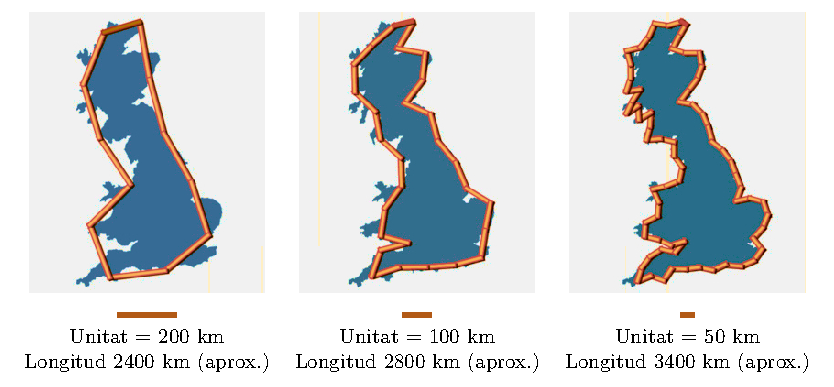
\includegraphics[width=0.75\textwidth]{img/img01_04_britain.pdf}
\caption{En aquesta imatge es pot observar el fenomen que Mandelbrot va observar respecte a la precisió en la mesura.}
\label{img01_04}
\end{figure}
Mentrestant va seguir treballant a l'IBM on se li va encarregar examinar les anomalies sonores que sofrien les transmissions electròniques. Allí, Mandelbrot va descobrir que, si es feia una gràfica amb les dades d'aquestes pertorbacions, es podia observar “autosimilitud” en totes les escales d'augment. El més curiós és que aquesta autosimilitud també podia apreciar-se en altres gràfics estadístics com per exemple els preus del cotó, les variacions de les cotitzacions de la borsa, les freqüències de les paraules en anglès i les fluctuacions dels líquids turbulents. Amb aquest fet, Mandelbrot va tornar a examinar els treballs de Gaston Julia, aconseguint construir la seva funció de Julia. Per tant, en combinar els treballs de Julia amb els seus estudis, aplicats a l’ordinador va assentar les bases del que més endavant serien els fractals.

Mandelbrot va batejar al seu descobriment amb el nom de fractal, paraula originària del llatí fractus. El significat de Fractus és trencat o irregular, definició que concorda amb el que va descobrir Mandelbrot i el motiu pel qual va utilitzar aquesta paraula. Temps després va batejar aquest corrent com geometria fractal, posicionant-se com el principal creador de la geometria fractal. L'any 1982 va publicar el seu llibre "Fractal Geometry of Nature", on explicava les seves investigacions i tesis sobre els fractals.

D’altra banda, Mandelbrot també es va interessar pels patrons del mercat financer. Investigant sobre aquestes va descobrir que els canvis de preu en el mercat no segueixen els convencionals patrons gaussians, sinó que seguien un esquema més proper als postulats per Lévy en els seus articles sobre el mercat. El concepte de fractals es va aplicar posteriorment a l'estudi dels mercats financers en el context dels fractals. 

A la fi de la dècada de 1980, Mandelbrot va utilitzar dades de ticks de Olsen \& Associates a Zúric per a aplicar la seva teoria dels fractals a l'estructura microestructural dels mercats. Aquesta col·laboració va donar lloc a la publicació dels primers treballs exhaustius sobre la llei d'escala en finances, que confirma la idea de Mandelbrot sobre la naturalesa fractal de la microestructura dels mercats.
\begin{figure}[!ht]
\centering
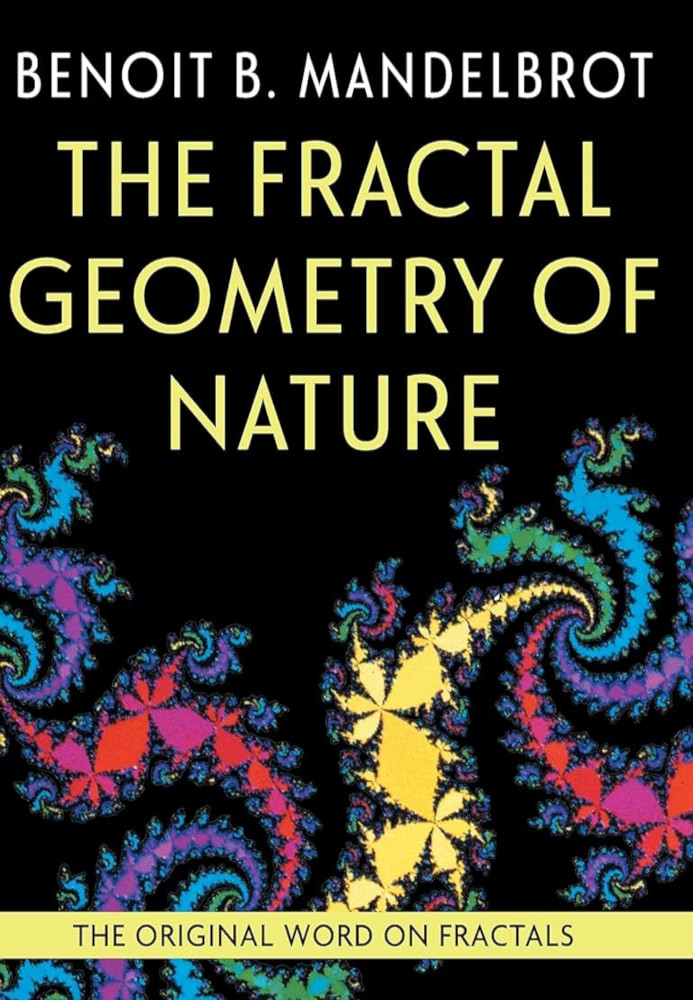
\includegraphics[width=0.35\textwidth]{img/img01_05_nature}
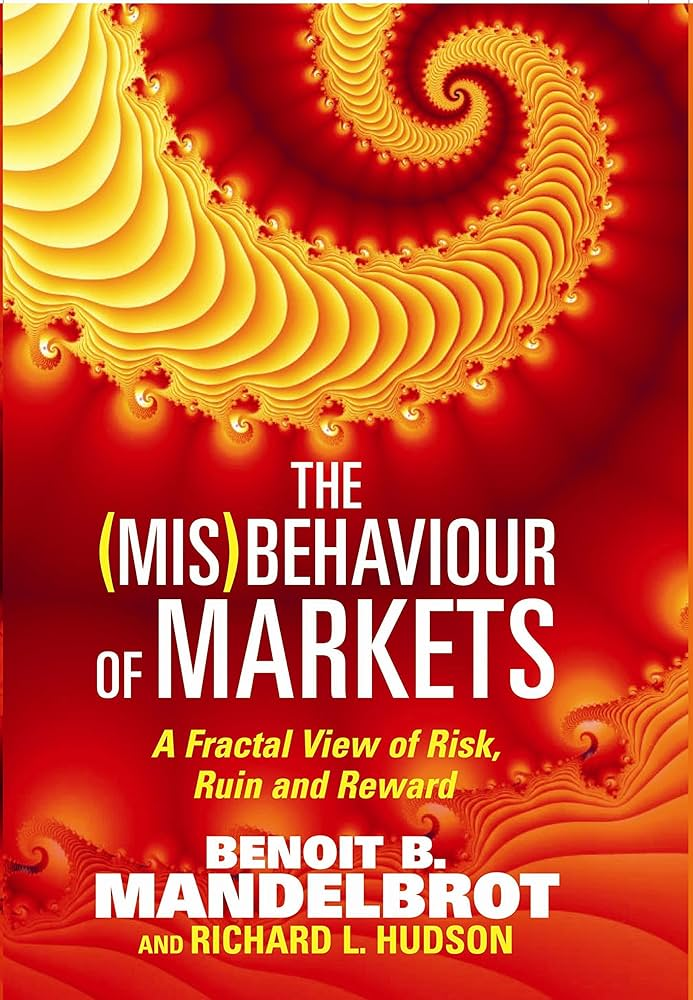
\includegraphics[width=0.35\textwidth]{img/img01_05_markets}
\caption{A l’esquerra el llibre ''Fractal Geometry of Nature'' (1982) i a la dreta ''The (Mis)Behavior of Markets'' (2004).}
\end{figure}
Anys després, l'any 1985 va ser guardonat amb el premi Barnard Medal for Meritorious Service to Science. Posteriorment, va guanyar la medalla Franklin. L’any 1987 va guanyar el premi Alexander von Humboldt, la medalla Steindal l'any 1988, la medalla Nevada al 91 i de més premis. Finalment, va morir l’any 2010 amb 85 anys a causa de càncer de pàncrees.

\chapter{FORMES FRACTALS}
\section{Conjunt de Cantor}
El conjunt de cantor, és un conjunt fractal batejat per Georg Cantor l'any 1883. Aquest conjunt és considerat com la primera estructura fractal registrada. El conjunt de Cantor destaca per ser un subconjunt de l'interval real $[0,1]$ i contradir la intuïció relativa de la mida d'un cos geomètric, és a dir, és un conjunt de mesura nul, però no és buit.
\subsection{Construcció}
Comencem amb l'interval tancat $[0,1]$, \cite[p.~66]{ChaosFractal}.
\begin{figure}[!ht]
\centering
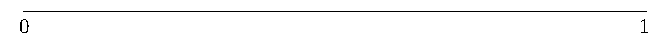
\includegraphics[scale=1]{img/img03_01_cantor.pdf}
\end{figure}

Ara treurem l'interval (obert) $\displaystyle\left(\frac{1}{3},\frac{2}{3}\right)$, és a dir, treurem el terç central de $[0,1]$, però no els nombres $\displaystyle\frac{1}{3}$ i $\displaystyle\frac{2}{3}$. Això deixa dos intervals $\displaystyle\left[0,\frac{1}{3}\right]$ i $\displaystyle\left[\frac{2}{3},1\right]$ de longitud $\displaystyle\frac{1}{3}$ cadascun i es completa un pas bàsic de la construcció.
\begin{figure}[!ht]
\centering
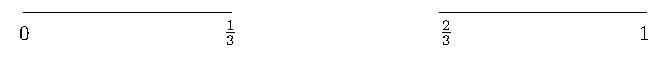
\includegraphics[scale=1]{img/img03_02_cantor.pdf}
\end{figure}

Ara repetim, ens fixem en els intervals restants $\displaystyle\left[0,\frac{1}{3}\right]$ i $\displaystyle\left[\frac{2}{3},1\right]$ i eliminem els seus terços mitjans, la qual cosa dona lloc a quatre intervals de longitud $\displaystyle\frac{1}{9}$.
\begin{figure}[!ht]
\centering
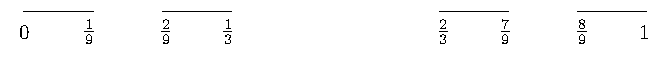
\includegraphics[scale=1]{img/img03_03_cantor.pdf}
\end{figure}

Continuem així. En altres paraules, existeix un procés de retroalimentació en el qual es genera una seqüència d'intervals (tancats): un després del primer pas, dos després del segon, quatre després del tercer, vuit després del quart, etc. (és a dir, $2^n$ intervals de longitud $\displaystyle\frac{1}{3^n}$ després de l'enèsim pas). La figura \ref{img03_04} mostra la seva construcció.

\begin{figure}[!ht]
\centering
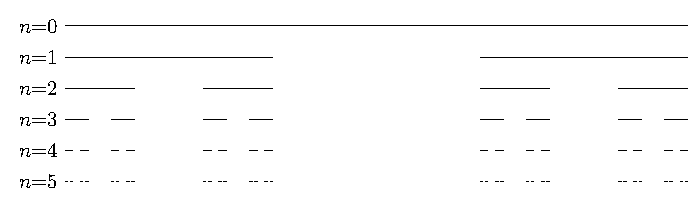
\includegraphics[scale=1]{img/img03_04_cantor.pdf}
\caption{Passos inicials del conjunt de Cantor.}
\label{img03_04}
\end{figure}
\section{Formes de Koch}
\subsection{La corba de Koch}
La corba de Koch \cite{Lopez:koch} és un fractal que va ser conegut l'any 1904 en un article anomenat: \emph{Sobre una corba continua que no té tangents i obtinguda per mètodes de la geometria elemental}.  L'article va ser publicat per Helge von Koch, un matemàtic suec (1870-1924), conegut per la teoria de nombres.  
\begin{figure}[!ht]
\centering
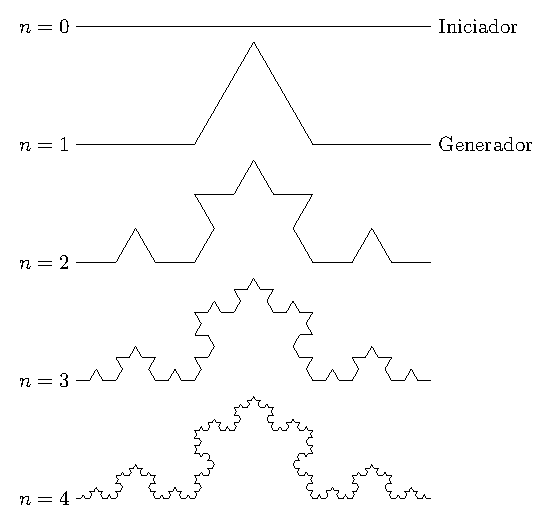
\includegraphics[scale=1]{img/img03_05_koch.pdf}
\caption{\textbf{Construcció de la corba de Koch}. La construcció de la corba de Koch es desenvolupa en etapes. En cada etapa, el nombre de segments de la línia augmenta per un factor de 4.}
\label{img03_05}
\end{figure}

La construcció de la corba comença amb una recta al pla, anomenada \textbf{iniciador}. Aquesta es divideix en terços i després se substitueix el terç central per un triangle equilàter sense la seva base, obtenint una nova figura de  quatre parts. D'aquesta figura obtinguda s'utilitzarà una reducció en les següents etapes anomenada \textbf{generador}. Ara, s'agafa cada un dels segments de la línia obtinguda i es reprodueix el generador en cada una de les parts i així successivament. En tot el procés de construcció es pot observar la característica d'autosimilitud, sent que cadascuna de les quatre parts en el  $k$-esim pas és de nou una versió reduïda de l'anterior (veure Figura \ref{img03_05}).
\subsection{El floc de neu de Koch}
Relacionat amb la corba de Koch trobem el floc de neu de Koch.  El floc de Koch, també anomenada illa o estrella de Koch, és una altra fractal obra de Helge von Koch. Es pot construir de dues formes, la primera i més senzilla (veure Figura \ref{img03_06}), és ajuntant 3 corbes de Koch pels seus extrems. Així s'obté el famós floc de Koch, una figura d'àrea finita i perímetre infinit. 

\begin{figure}[!ht]
\centering
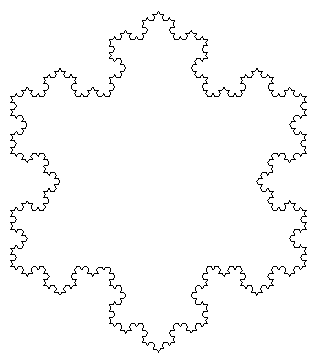
\includegraphics[scale=1]{img/img03_06_koch.pdf}
\caption{\textbf{El floc de neu de Koch}. Ajuntem 3 corbes de Koch pels seus extrems.}
\label{img03_06}
\end{figure}
%Tammbé, es pot construir utilitzant un triangle equilàter com iniciador (veure Figura \ref{img03_07}), afegint triangles de longitud lateral $\displaystyle\frac{1}{3}$ al voltant de l'iniciador, repetint aquest procés, similar a una seqüència recursiva.
%
%Després de la primera iteració, el nombre de nous triangles afegits augmenta en un factor de 4 en cada pas. De la mateixa manera, l'àrea d'aquests triangles disminueix en un factor de 9 per cada pas.

L'altra manera de desenvolupar el floc de Koch començaria amb un triangle equilàter (omplert) de longitud lateral igual a $L$. Aquest triangle serà en el nostre iniciador. 

\begin{figure}[!ht]
\centering
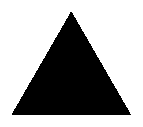
\includegraphics[scale=1]{img/img03_06_koch_01.pdf}
\end{figure}

En el segon pas, al terç mitjà de cada costat del triangle afegim un nou triangle equilàter de longitud lateral igual a $\displaystyle\frac{1}{3}L$. D'aquesta manera obtenim el generador.

\begin{figure}[!ht]
\centering

\includegraphics[scale=1]{img/img03_06_koch_02.pdf}
\end{figure}
\newpage
A continuació, al terç mitjà de cada costat del generador afegim triangles equilàters de longitud lateral  igual a $\displaystyle\frac{1}{3}\left(\frac{L}{3}\right)=\frac{L}{9}$.
\begin{figure}[!h]
\centering
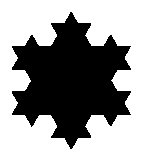
\includegraphics[scale=1]{img/img03_06_koch_03.pdf}
\end{figure}

Finalment, repetim aquest procés de manera seqüencial fins a obtenir la Figura \ref{img03_07} 

\begin{figure}[!ht]
\centering
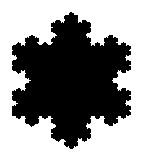
\includegraphics[width=0.5\textwidth]{img/img03_06_koch_04.pdf}
\caption{\textbf{El floc de neu de Koch}. 5 iteracions del floc de Koch.}
\label{img03_07}
\end{figure}

\begin{figure}[!ht]
\centering

\includegraphics[scale=.5]{img/img03_08.pdf}
\caption{\textbf{Flocs naturals}. El floc de neu de Koch comparteix similitud amb els flocs de la vida real.}
\end{figure}

\section{Formes de Sierpiński}
Un dels grans contribuïdors al camp dels fractals fou Sierpiński. Wacław Sierpiński fou un matemàtic polonès (1883-1969), amb grans contribucions dins de les matemàtiques com la teoria de conjunts i la de números. També es va interessar pels fractals, molt abans que Mandelbrot creés el terme fractal. Sierpiński va construir diversos objectes fractals:
\begin{itemize}
\item Triangle de Sierpiński
\item Catifa de Sierpiński
\item Corba de Sierpiński
\item Tetraedre de Sierpiński
\item Piràmide de Sierpiński
\end{itemize}
\subsection{Triangle de Sierpiński}
El més conegut de les fractals de Sierpiński, i la seva obra magna, és el triangle de Sierpiński \cite{ChaosFractal}. Aquest triangle es forma des d'un triangle equilàter al qual se li va removent recursivament triangles més petits fora del centre. A diferència de les altres formes de Sierpiński, la seva existència és milers d'anys a Sierpiński, ja que era utilitzat per antigues civilitzacions com a patró de decoració. Així i tot, va ser batejada com ''de Sierpiński'' pel fet que ell va ser el primer a estudiar les seves propietats matemàtiques.

La construcció geomètrica del triangle Sierpiński és la següent \cite[p.~76]{ChaosFractal}. Comencem amb un triangle ple en el pla i després li apliquem un esquema repetitiu d'operacions. Després es localitza els punts mitjans dels seus tres costats i s'ajunten amb els antics vèrtexs del triangle original, aquests punts mitjans defineixen quatre triangles congruents dels quals eliminem el del centre. Això completa el pas bàsic de la construcció. En altres paraules, després del primer pas tenim tres triangles congruents els costats dels quals tenen exactament la meitat de la grandària del triangle original i que es toquen en tres punts que són vèrtexs comuns de dos triangles contigus.
\begin{figure}[!ht]
\centering
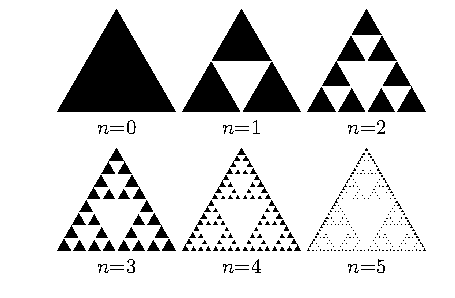
\includegraphics[scale=1]{img/img03_09_sierpinski.pdf} 
\caption{\textbf{Triangle de Sierpiński.} Els passos bàsics de construcció del triangle de Sierpiński.}
\label{img03_09}
\end{figure}

Ara seguim el mateix procediment amb els tres triangles restants i repetim el pas bàsic tantes vegades com ho desitgem. És a dir, comencem amb un triangle i després produïm 3, 9, 27, 81, 243$\ldots$ triangles (veure Figura \ref{img03_09}), cadascun dels quals és una versió escalada exacta dels triangles en el pas anterior.  El triangle de Sierpiński és el conjunt de punts en el pla que queden si es duu a terme aquest procés infinitament sovint.  La característica de l'autosimilitud i recursivitat són presents  en el procés de construcció, és a dir, cadascuna de les tres parts del pas és una versió lluïda - per un factor de 2 - de tota l'estructura del pas anterior.

\subsection{Relació entre triangles: Sierpiński i Pascal} 
El triangle de Sierpiński és un objecte que ha aconseguit plasmar-se cap a altres conceptes dins de les matemàtiques.  Tan així, que el triangle del matemàtic polonès està relacionat amb un altre triangle famós, el triangle de Pascal/Tartaglia.  

El triangle de Pascal, o també anomenat de Tartaglia \cite[p.~80]{ChaosFractal}, es defineix com una piràmide numèrica en la qual es troben representats els coeficients binominals de l'equació \ref{eq_pascal}.  La seva construcció comença amb el número 1 al vèrtex superior i s'expandeix cap avall amb la resta de nombres de manera seqüencial. D'aquesta manera, el triangle hauria de tenir l'estructura següent:

\begin{figure}[!ht]
\centering
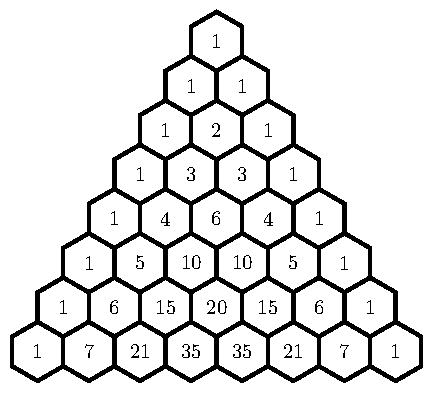
\includegraphics[scale=.8]{img/img03_10_b_sierpinski.pdf}
\caption{\textbf{Triangle de Pascal/Tartaglia}. Il·lustració de les primeres 8 files del triangle.}
\end{figure}
 
El disseny del triangle de Pascal s'obté amb la següent fórmula:
\begin{align}\label{eq_pascal}
c(n,k)=\binom{n}{k}=\frac{n!}{(n-k)!k!}, \qquad n\in \mathbb{N},\quad k=0,\dots,n.
\end{align}
Aquí, $n$ i $k$ representen el número files i columnes que té el triangle respectivament. En la Taula \ref{tab03_05_01} es poden observar les 4 primeres files del triangle de pascal.

\begin{table}[!ht]
\centering
{\UseRawInputEncoding
\begin{tabular}{|c|c|c|c|}
\hline
$n$ & $k$ & $c(n,k)$ & valors\\
\hline
0 & 0 & c(0,0) & 1 \\
1 & 0,1 & c(1,0), c(1,1) & 1, 1 \\
2 & 0,1,2 & c(2,0), c(2,1), c(2,2) & 1, 2, 1 \\
3 & 0,1,2,3 & c(3,0), c(3,1), c(3,2), c(3,3) & 1, 3, 3, 1 \\
\hline
\end{tabular}
}
\caption{Les primeres 4 files del triangle de Pascal.}
\label{tab03_05_01}
\end{table}

Doncs bé, una característica del triangle de Pascal és que es pot obtenir el triangle de Sierpiński dins d'aquest si s'utilitza un codi de colors per diferenciar els nombres parells dels imparells (veure Figura \ref{img03_10}).  

També es pot formar utilitzant un codi de colors basant-se en els nombres divisors d'un nombre $m\in\mathbb{N}$ (veure Figura \ref{img03_11}).

\begin{figure}[!ht]
\centering
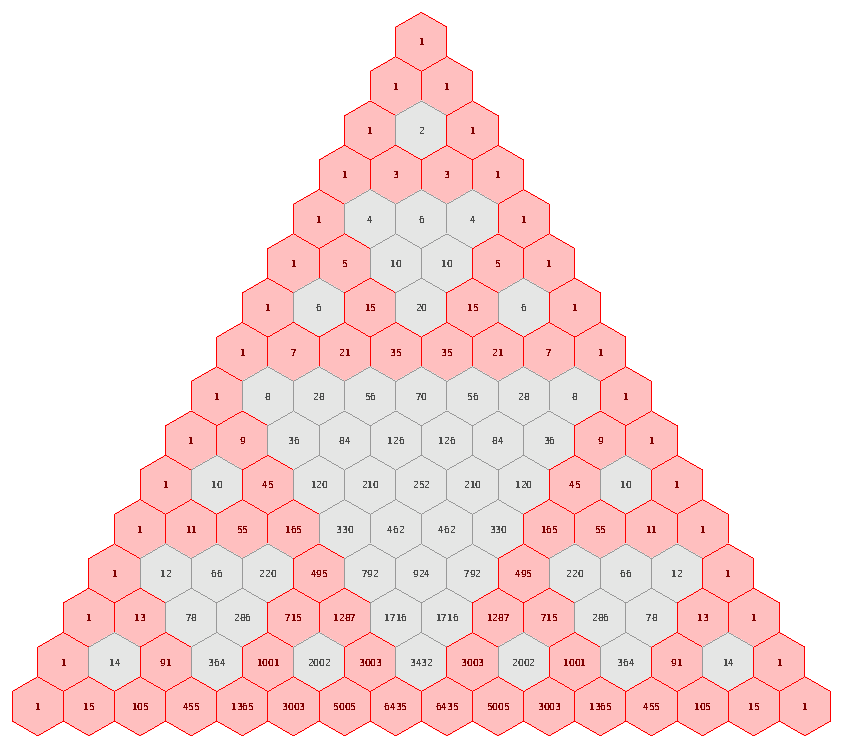
\includegraphics[scale=1]{img/img03_10_sierpinski.pdf} 
\caption{\textbf{Codificació de color.} Codificació per colors d'entrades paris (grises) i imparelles
(vermelles) en el triangle de Pascal amb 16 files.}
\label{img03_10}
\end{figure}

\begin{figure}[!ht]
\begin{center}
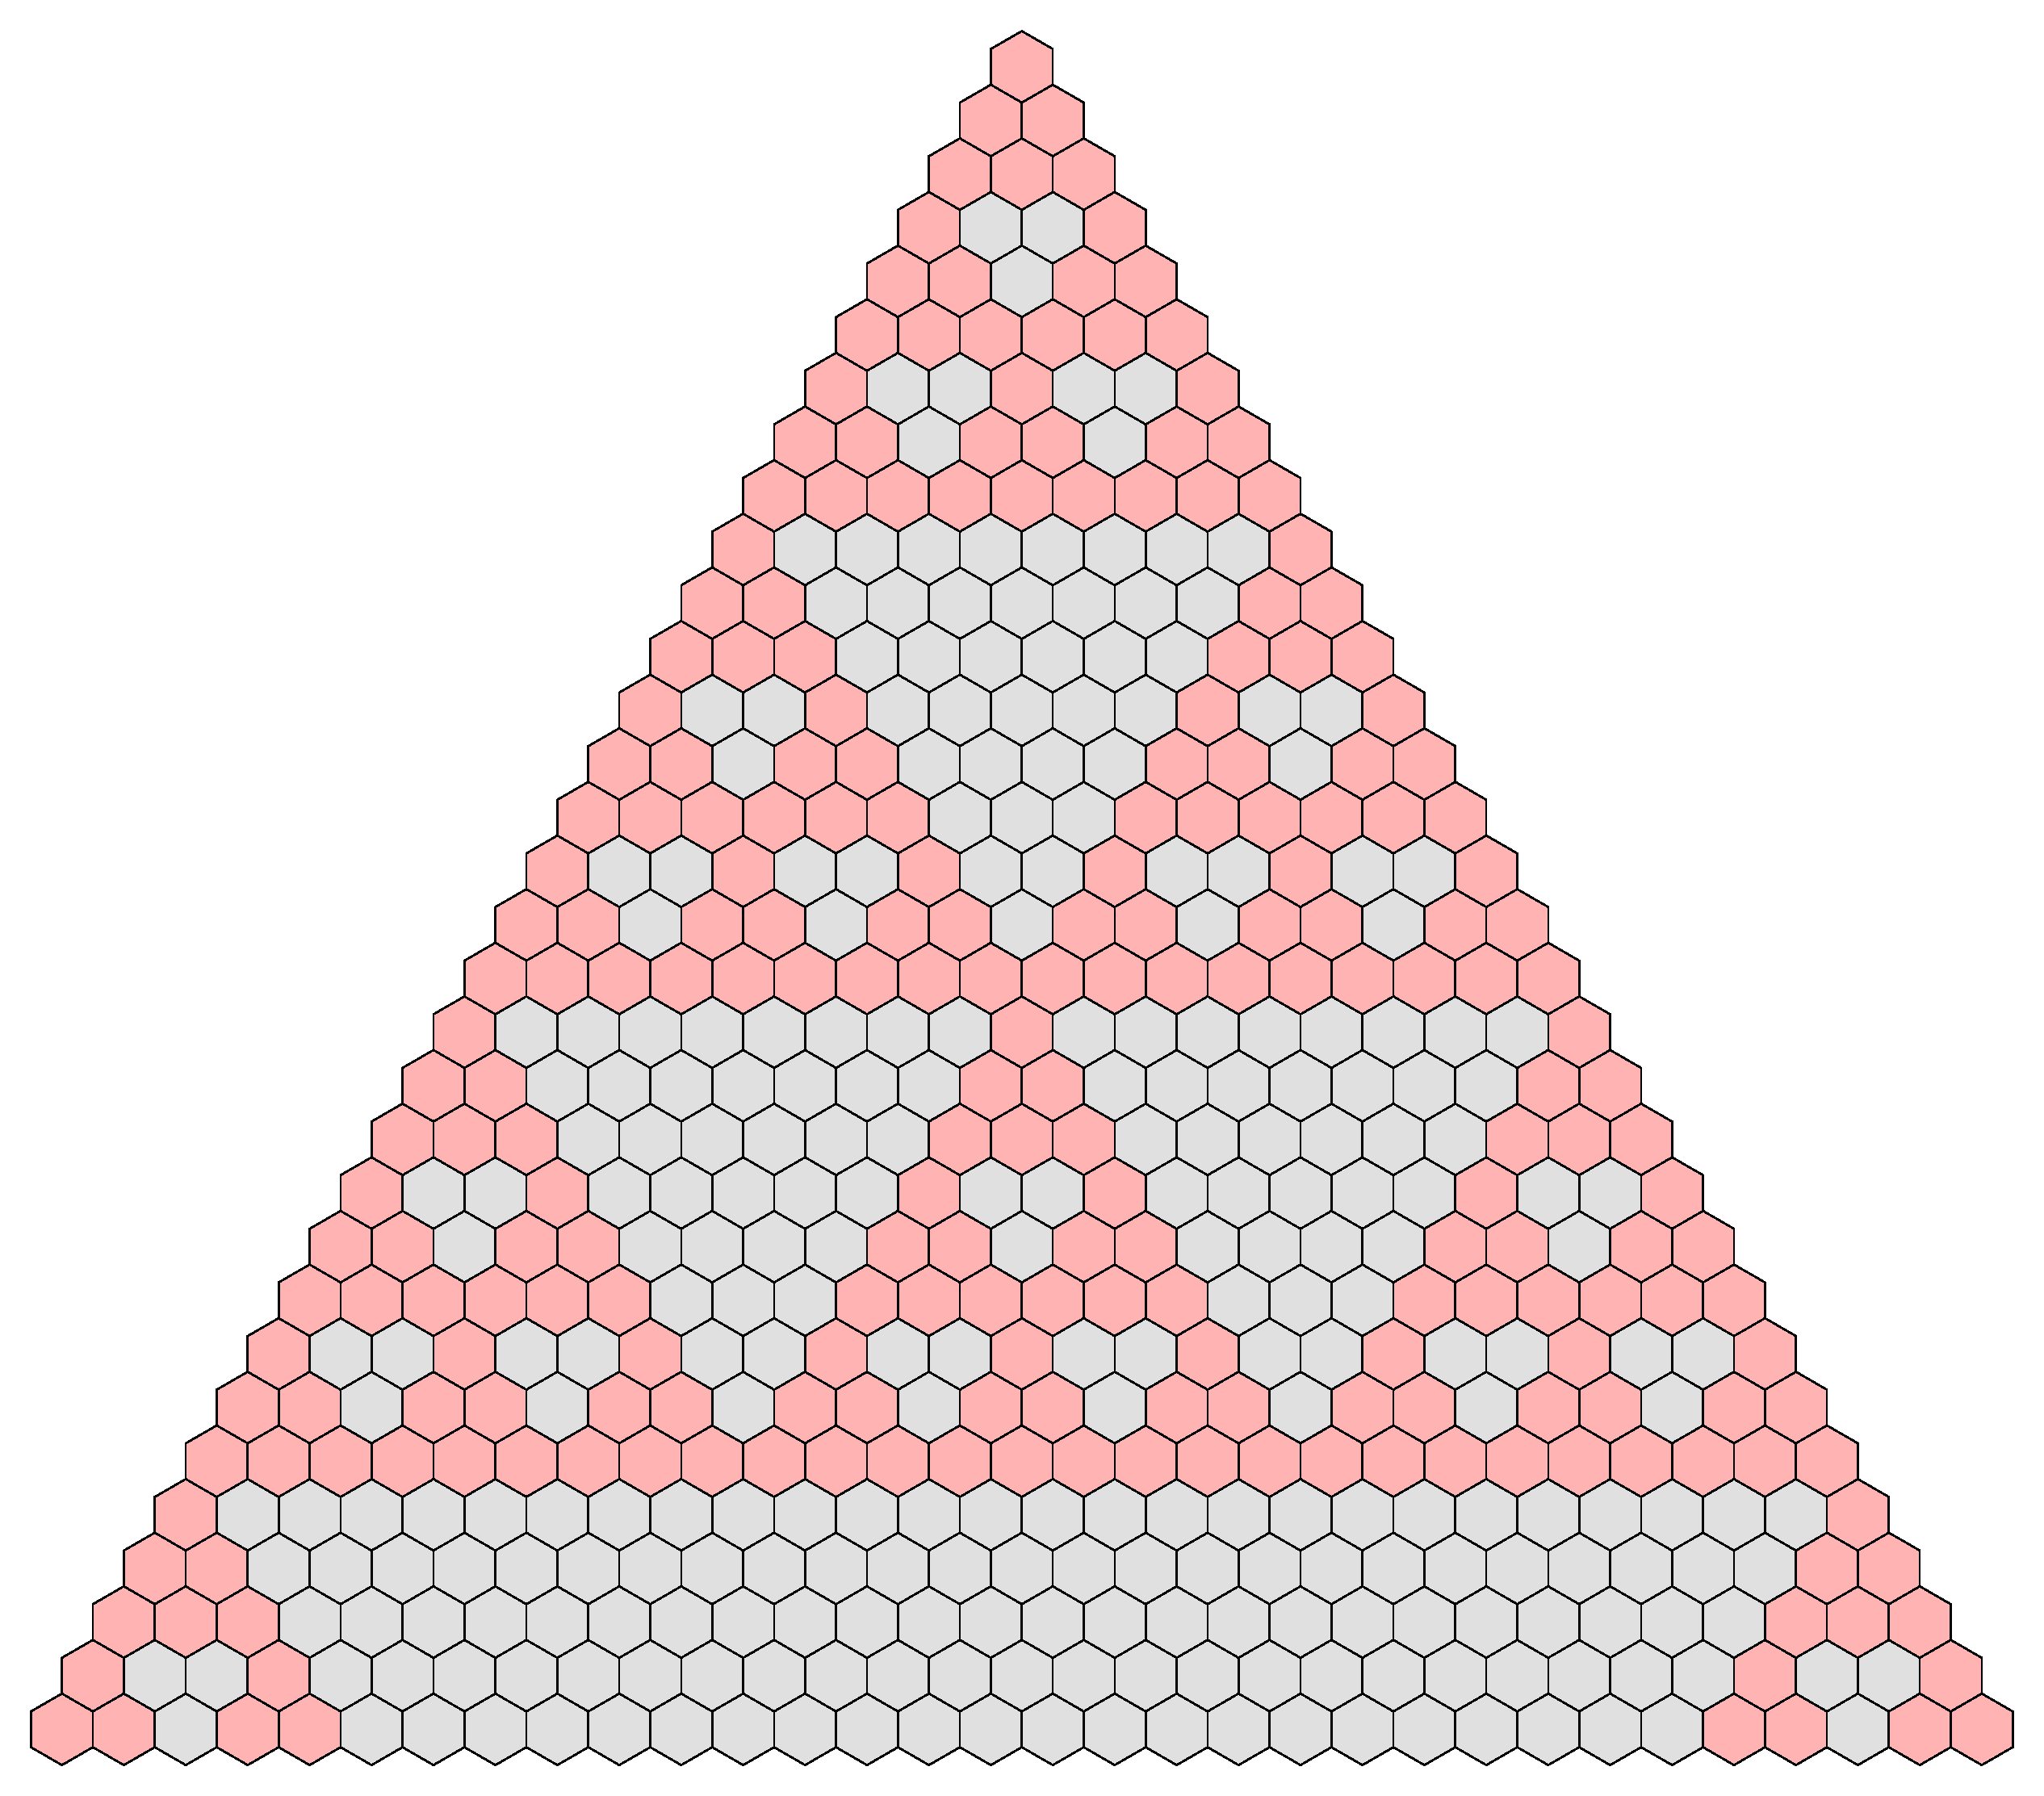
\includegraphics[width=0.4\textwidth]{img/img03_11_01_pascal.pdf} 
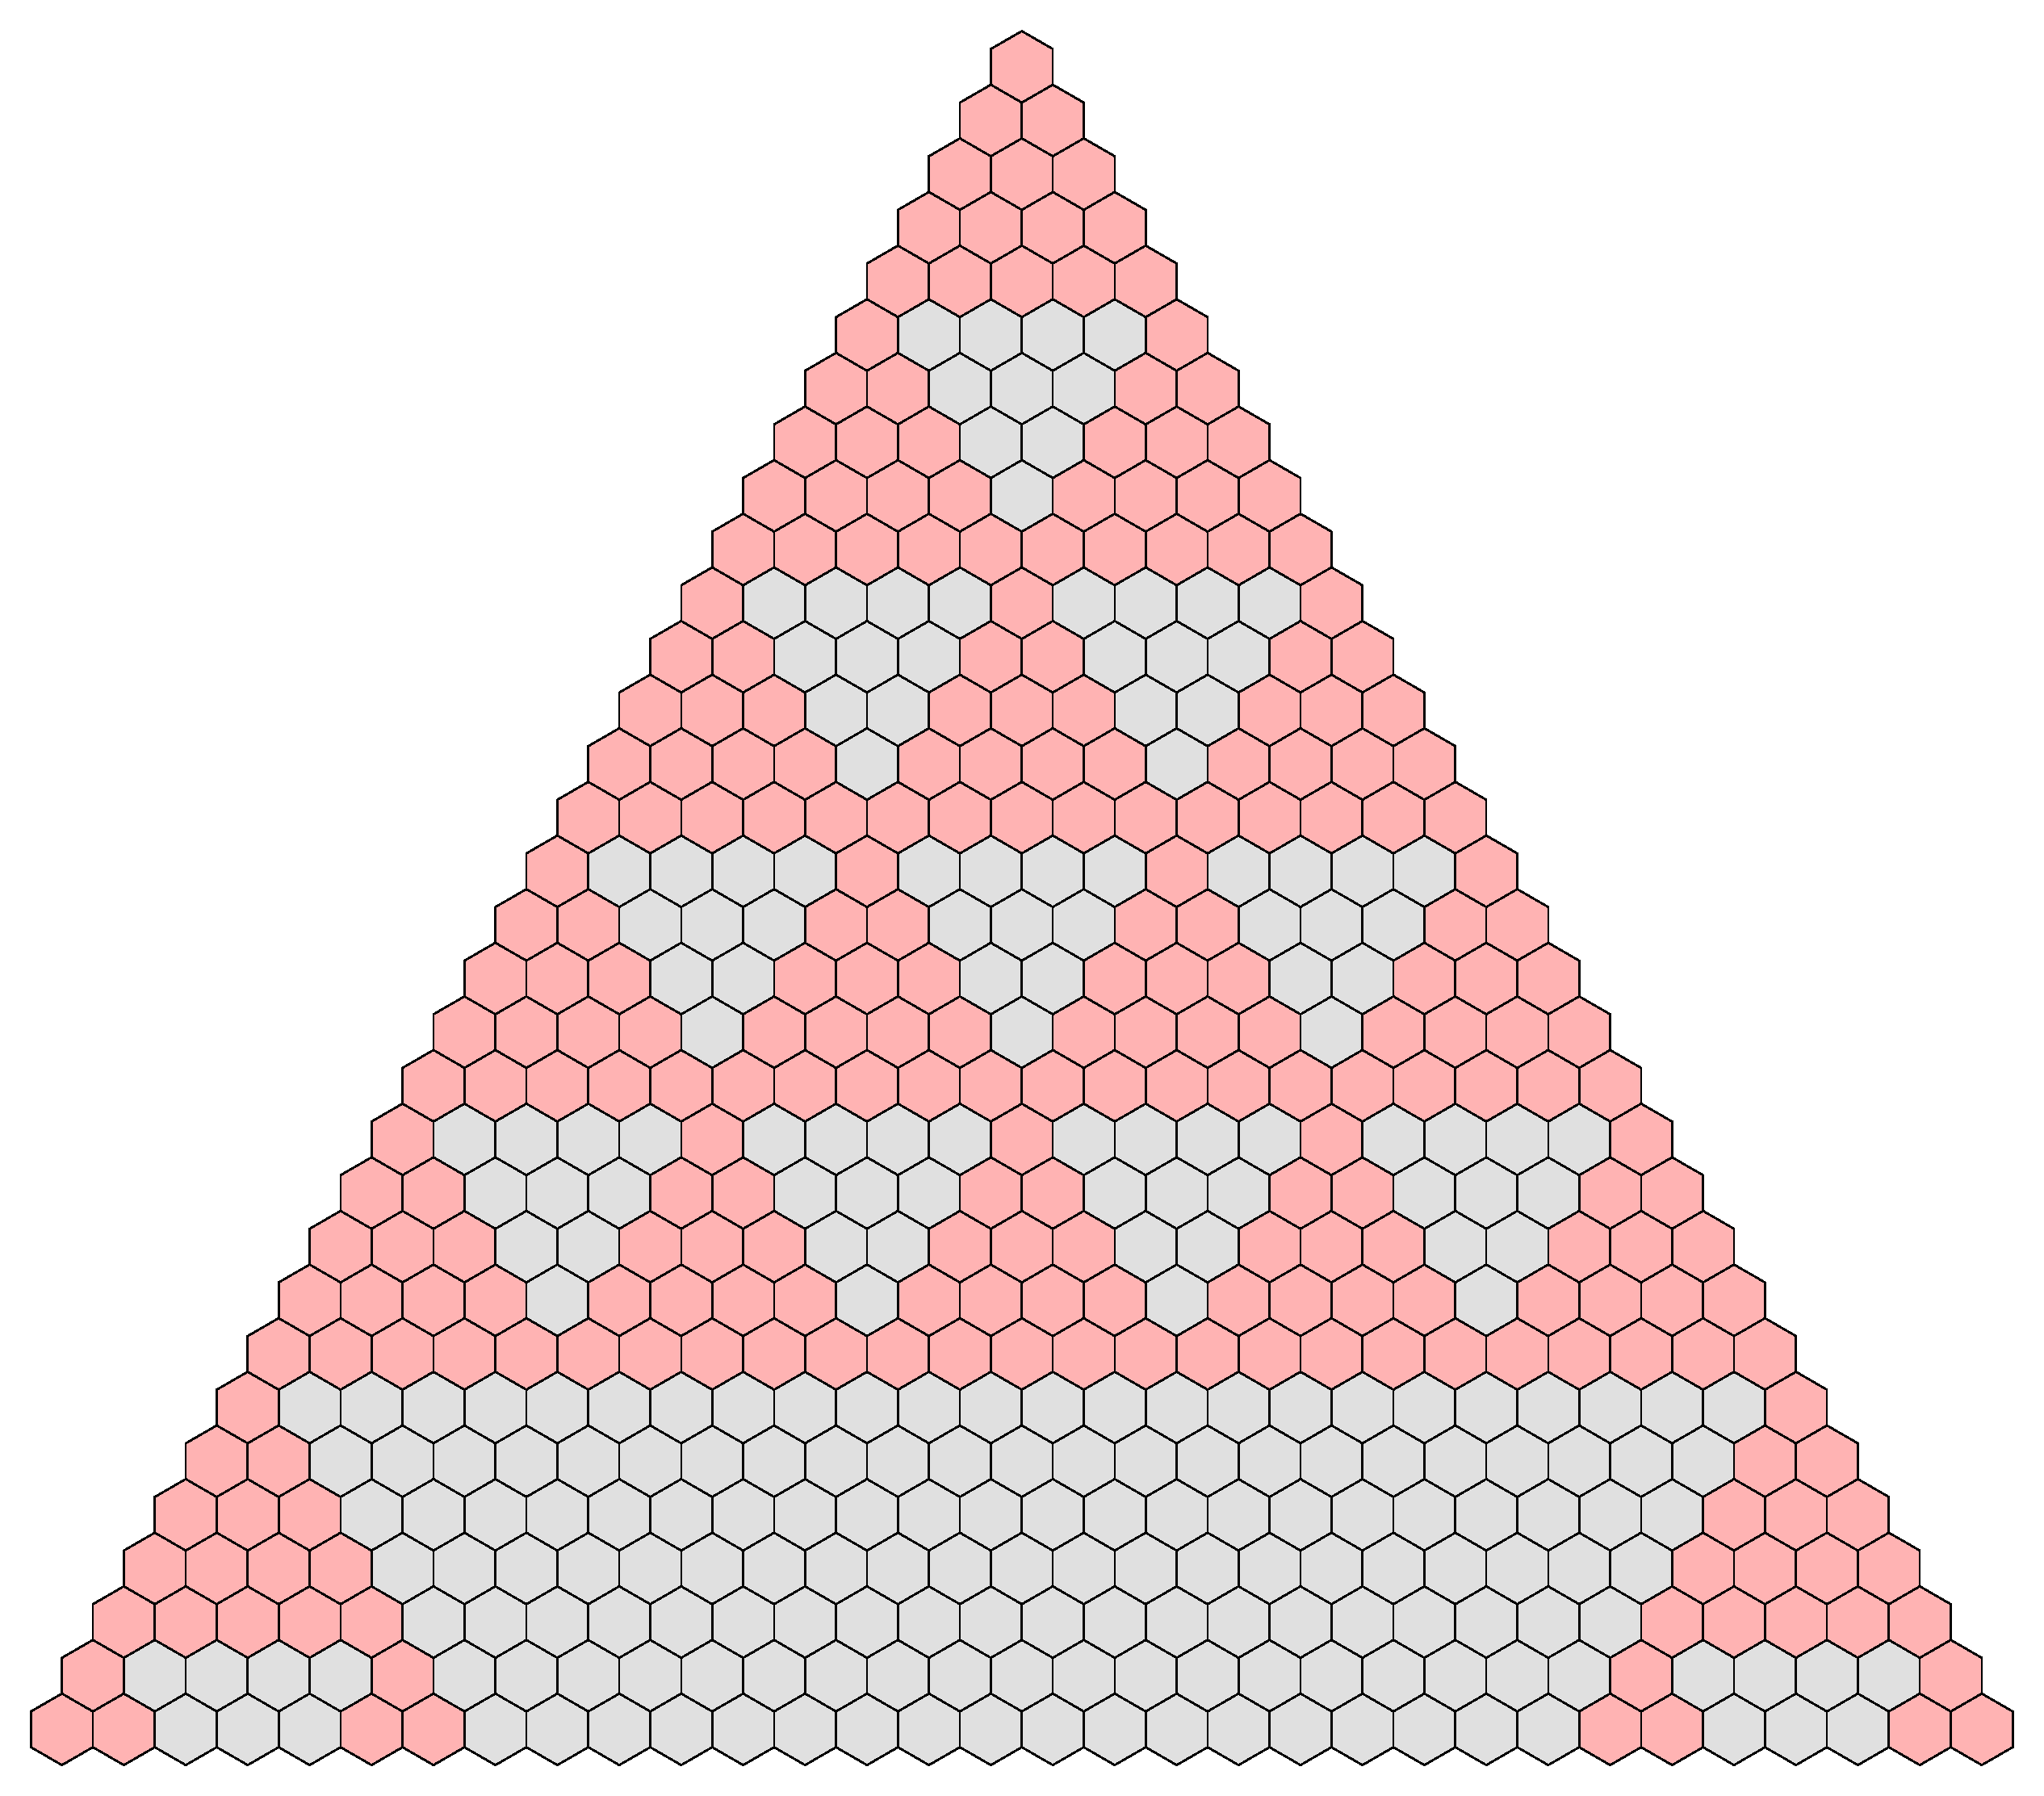
\includegraphics[width=0.4\textwidth]{img/img03_11_02_pascal.pdf} 
\end{center}
\caption{\textbf{Codi de colors del triangle de Pascal.} Les cel·les grises indiquen la divisibilitat entre 3 (a l'esquerra) i 5 (a la dreta).}
\label{img03_11}
\end{figure}
\newpage
\subsection{Catifa}
La catifa és el següent fractal que va crear Sierpiński, l'any 1916 \cite[p.~79]{ChaosFractal}. Aquesta figura es construeix a partir d'un quadrat en el pla, el qual subdividim en 9 quadrats més petits de costat $\displaystyle\frac{1}{3}$ del costat original, eliminant també el del centre. Després, aquest procés es repeteix amb cadascun dels quadrats successivament. Per cada iteració, el nombre de quadrats es multiplica per 8 i cada quadrat sempre tindrà de mida $\displaystyle\frac{1}{3}$ del quadrat de la iteració anterior.

\begin{figure}[!ht]
\centering
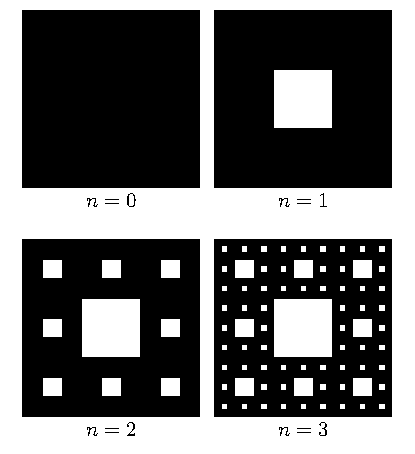
\includegraphics[scale=1]{img/img03_12_sierpinskiCarpet.pdf} 
\caption{\textbf{Catifa de Sierpiński.} Els passos bàsics de construcció de la catifa de Sierpiński.}
\end{figure}
\subsection{Tetraedre}
Fins ara hem vist fractals que es representen al pla (d'entre 1 a 2 dimensions). Ara bé, no tots els fractals  són ''plans'', existeixen diversos fractals amb dimensió irracional major a 2. Amb aquesta premissa apareix el tetraedre o piràmide de Sierpiński \cite[p.~129]{KitchenScience}. Aquesta és una representació tridimensional del triangle de Sierpiński (veure Figure \ref{img03_13}).
\begin{figure}[!ht]
\centering
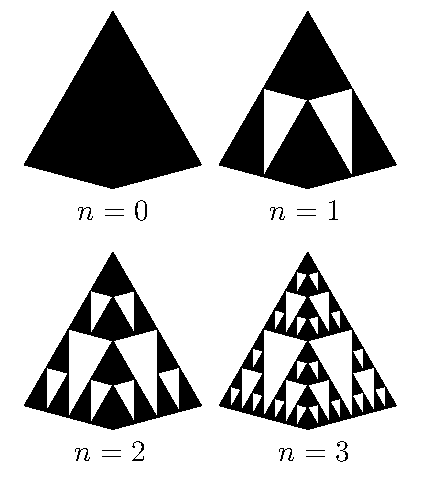
\includegraphics[scale=1]{img/img03_13_sierpinskiTetra.pdf} 
\caption{\textbf{Tetraedre de Sierpiński.}}
\label{img03_13}
\end{figure}
El seu procés de construcció es realitza partint d'un tetraedre. Sobre cadascuna de les seves cares, marquem els punts mitjans de les arestes. En unir-les s'elimina la part central. D'aquesta manera obtenim un objecte format amb quatre tetraedres que seria la 1a iteració. Per a obtenir les següents iteracions es repeteix el mateix procés en cadascun dels quatre tetraedres obtenint un nou objecte.
\subsection{Esponja de Menger}
Un altre fractal amb dimensió superior a 2 és l'anomenada esponja de Menger \cite[p.~106]{ChaosFractal}. L'esponja de Menger és un fractal quasi tridimensional, batejat així pel matemàtic austríac Karl Menger, que el va descriure l'any 1926.

La seva construcció és semblant a la de la catifa de Sierpiński, però, amb un cos tridimensional. Es comença amb un cub sòlid, el qual és perforat repetidament en forats quadrats cada cop més petits. Amb cada iteració els forats tenen una mesura de $\displaystyle\frac{1}{3}$ dels forats de la iteració prèvia.
\begin{figure}[!ht]
\centering
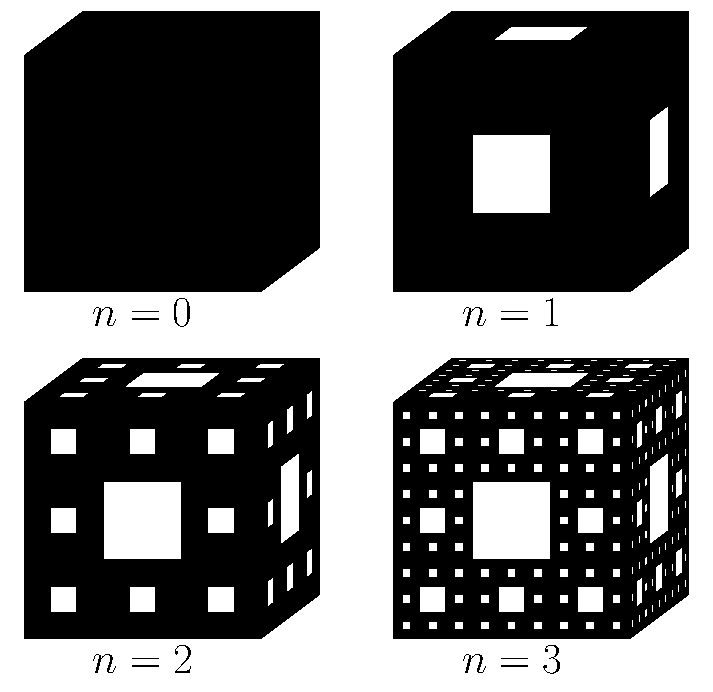
\includegraphics[scale=0.6]{img/img03_14_menger.pdf}
\caption{\textbf{Construcció de l'esponja de Menger.} }
\end{figure}
\section{Corba de drac}
La corba de drac \cite{Lopez:dragon} es una corba fractal que va ser obtinguda mitjançant un procés iteratiu. Va ser observada per primera vegada a la NASA pels fisics Juan Heighway y Guillermo Harter, es per això, que també la corba es anomenada com el Drac d’Heighway-Harter. 

\begin{figure}[!ht]
\centering
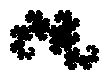
\includegraphics[width=1\textwidth]{img/img03_dragon_curve.pdf}
\caption{\textbf{La corba de Drac.} }
\end{figure}
Entre les seves propietats tenim les següents:
\begin{itemize}
\item La corba de drac té diverses variants, que es poden generar al cambiar l’angle de gir, també si es generen més d’una corba de drac (Tetradrac y el drac bessó).
\end{itemize}
\subsection{Construcció de la corba drac}
Per a la seva construcció utilitzarem un triangle isòsceles sense base com iniciador. Després, generem un triangle orientat cap a dalt, en el costat esquerre del triangle, i un altre triangle orientat cap avall al costat dret, obtenint el generador. Aquest procés es repeteix seqüencialment en tots els triangles isòsceles sense base de la figura anterior.
\begin{figure}[!ht]
\centering
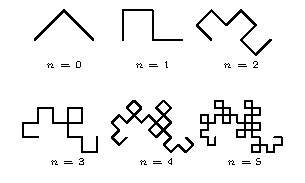
\includegraphics[width=0.65\textwidth]{img/img03_dragon_curve_01.pdf}
\caption{\textbf{Construcció de la corba de Drac.} }
\end{figure}
\section{Corbes que omplen l'espai}
L’any 1890, el matemàtic Giuseppe Peano \cite{Asociacionceat}, publica l'article ''Sur une courbe qui remplit toute une aire plane'', conegut en català com a ''corbes que omplen l’espai''. En aquest article, Peano explicava el descobriment d'una corba contínua, la qual tenia la peculiaritat d'\,''omplir'' tot el pla, aquesta corba, seria batejada com corba de Peano l’any 1891. Un any després David Hilbert va fer una ''variant'' d'aquesta corba que seria coneguda com la corba de Hilbert.

Aquestes corbes que omplen l'espai, es construeixen mitjançant successions de corbes contínues sense interseccions, convergint en sola corba, que també s'anomena corba límit, la qual, passa per qualsevol punt de la superfície. És a dir, aquestes corbes són infinites i continues.
\subsection{Construcció d'una corba de Peano}
La construcció de la corba de Peano \cite[p.~92]{ChaosFractal} comença amb un segment de línia recta amb longitud 1, que serà l'iniciador ($k$). En aquest recte es tracen nous segments fins que queden 9 segments amb mesura $l = \displaystyle\frac{k}{3}$, com s'indica a la Figura \ref{img03_14} (generador). Aquest procediment se'n va repetint en aquests 9 segments i així  indefinidament en cada generador que es va obtenint com es mostra a la Figura \ref{img03_14}.  

\begin{figure}[!ht]
\centering
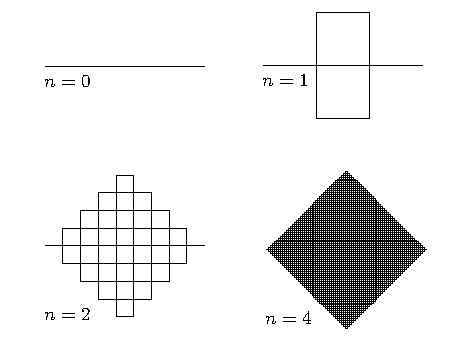
\includegraphics[width=0.7\textwidth]{img/img03_peano_00.pdf}
\caption{\textbf{Construcció de la corba de Peano en 4 pasos.} L'iniciador ($n = 0$) i tres generadors o iteracions ($n = 1, 2, 4$).}
\label{img03_14}
\end{figure}

\subsection{Altres corbes de Peano/corbes que omplen l'espai}
\begin{table}[!ht]
\centering
{\UseRawInputEncoding
{\tabulinesep=1.25mm
\begin{tabu}{|c|p{4cm}|}
\hline
Nom & Representaci�\\
\hline
Corba de Hilbert & 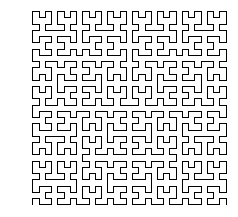
\includegraphics[valign=c, width=3.75cm]{img/img03_hilbert_curve.pdf}\\
\hline
Corba de Moore & 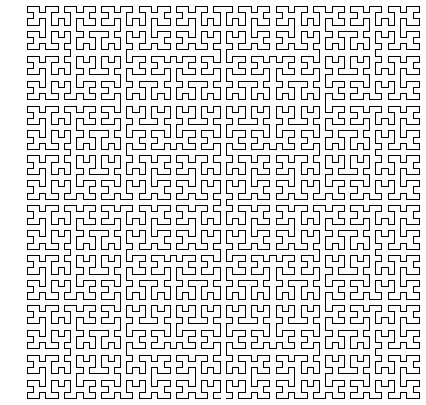
\includegraphics[valign=c, width=3.75cm]{img/img03_moore_curve.pdf}\\
\hline
\end{tabu}}
%\caption{Altres corbes que omplen l'espai o de peano. Ambdues tenen dimensi� fractal 2.}
}
\caption{Altres corbes que omplen l'espai o de Peano. Ambdues tenen dimensió fractal 2.}
\end{table}
\newpage
\section{Conjunt de Julia}
Els conjunts de Julia \cite{JuliaMandelbrot}, batejats així en honor al matemàtic Gaston Julia, són una agrupació de fractals que s'obtenen en estudiar el comportament dels nombres complexos en ser iterats per una funció. La característica d'aquests conjunts es troba en el fet que la seva funció $f$ només es troba constituïda per aquelles iteracions del nombre complex on els punts de la funció tenen una distribució ''caòtica''.

Un dels conjunts de Julia més coneguts, és aquell que s'obté de la funció quadràtica següent:
\begin{align}\label{eq02_julia}
f_{c}(z)=z^2 + c.
\end{align}

On utilitzem un nombre $c$ concret, el qual utilitzem per construir una succesió de nombres, és a dir, fem iteracions d'aquesta funció:
\begin{align*}
z_0 &= z \\
z_1 &= f_{c}(z_0)= z_{0}^2 + c \\
z_2 &= f_{c}(z_1) =z_{1}^2+c \\
& \vdots \\
z_n &= f_{c}(z_{n-1}) =z_{n-1}^2+c 
\end{align*}

\paragraph*{El cas especial $c=0$.} Un cas especial es per a $c$ = 0, on $f_{0}(z) = z^{2}$ és la funció més bàsica i el punt de sortida a un increïble catàleg de bells conjuntes fractals de Julia. 

\begin{table}[!ht]
\centering
{\UseRawInputEncoding
\resizebox{\textwidth}{!}{
\begin{tabular}{|l|rr|rr|rr|}
\hline
$z$ & \multicolumn{2}{c|}{�rbita 1} & \multicolumn{2}{c|}{�rbita 2} & \multicolumn{2}{c|}{�rbita 3}\\
\hline
 & successi� & m�dul & successi� & m�dul & successi� & m�dul\\
\hline
$z_0$ & 0.8863+0.1563$i$ & 0.9000 & 0.9781+0.2079$i$ & 1.0 & 0.931+0.5375$i$ & 1.0750 \\
$z_1$ & 0.7612+0.277$i$ & 0.8100 & 0.9135+0.4067$i$ & 1.0 & 0.5778+1.0008$i$ & 1.1556 \\
$z_2$ & 0.5026+0.4217$i$ & 0.6561 & 0.6691+0.7431$i$ & 1.0 & -0.6677+1.1566$i$ & 1.3355 \\
$z_3$ & 0.0747+0.4239$i$ & 0.4305 & -0.1045+0.9945$i$ & 1.0 & -0.8917-1.5445$i$ & 1.7835 \\
$z_4$ & -0.1741+0.0634$i$ & 0.1853 & -0.9781-0.2079$i$ & 1.0 & -1.5904+2.7546$i$ & 3.1808 \\
$z_5$ & 0.0263-0.0221$i$ & 0.0343 & 0.9135+0.4067$i$ & 1.0 & -5.0587-8.762$i$ & 10.1174 \\
$z_6$ & 0.0002-0.0012$i$ & 0.0012 & 0.6691+0.7431$i$ & 1.0 & -51.1813+88.6487$i$ & 102.3627 \\
\hline
\end{tabular}}
}
\caption{\textbf{Dinàmica de $z\rightarrow z^2$.} La iteració de tres punts inicials usant l'operació d'elevació al quadrat simple $z\rightarrow z^{2}$.}
\label{tab03_02_01}
\end{table}

La Taula \ref{tab03_02_01} mostra el comportament dinàmic de tres nombres complexos. En tots els casos observem que les successions de les òrbites giren al voltant de l'origen. No obstant això, el punt inicial de l'òrbita 1 que es troba dins del cercle unitari produeix una successió que convergeix cap a l'origen, el punt inicial de l'òrbita 2 que es troba exactament en el cercle unitari produeix una successió que roman allí per sempre, i el punt inicial de l'òrbita 3 exterior al cercle unitari produeix una successió que escapa a l'infinit, és a dir, el valor absolut de les iteracions augmenta cada vegada més (veure Fgura \ref{img03_01}). 

\begin{figure}[!ht]
\centering
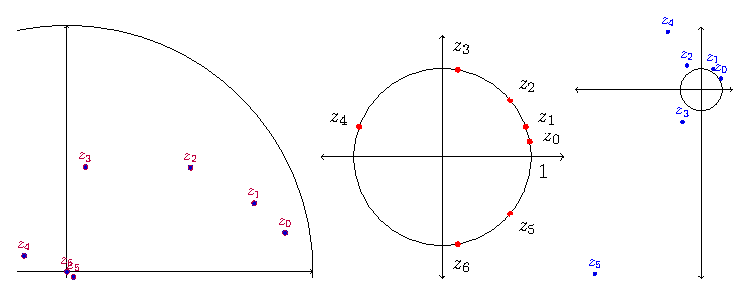
\includegraphics[scale=1]{img/img03_01_prisioners.pdf}
\caption{\textbf{Iterant $z \rightarrow z^{2}$.} S'iteren els tres punts inicials de la Taula \ref{tab03_02_01}.}
\label{img03_01}
\end{figure}

\paragraph*{Conjunt de Presoners i Fuita.}
Això ens porta a una important dicotomia dinàmica: el pla complex de valors inicials $z_0$ se subdivideix en dos subconjunts.
\begin{itemize}
\item \textbf{El conjunt de fuita $E$.} El qual recull els punts $z_0$ per als quals la seva iteració s'escapa a l'infinit.
\item \textbf{El conjunt de presoners $P$.} Recull els punts $z_0$ per als quals tots els valors de la seva iteració romanen en una regió delimitada.
\end{itemize}
Observi que $P$ és el disc al voltant de 0 amb radi 1 i que $E$ és l'exterior d'aquest disc. La frontera entre $E$ i $P$ és el cercle unitari. Per tant, a aquesta frontera se'l denomina el \textbf{conjunt de Julia} i al conjunt de presoners $P$ el \textbf{conjunt ple de Julia}.

\paragraph{Conjunts de Julia per a la família quadràtica $f_{c}(z)=z^{2}+c$.}
El cas especial $z\rightarrow z^{2}$ és la porta d'entrada a un increïble zoològic de bells conjuntes fractals de Julia. Un departament d'aquest zoològic de conjunts de Julia es construeix sobre la iteració de $f_{c}(z)=z^{2}+c$, on $c$ és un paràmetre complex. El conjunt de Julia de $z\rightarrow z^{2}$ està just en el centre d'aquesta classe; $c=0$. Com el cercle unitari és la frontera del conjunt de fuita per a $f_{0}(z)=z^{2}$, els altres conjunts de Julia són les fronteres del conjunt de fuita de $z\rightarrow z^{2}+c$. Per tant, la frontera comuna entre $E_c$ i $P_c$ és el conjunt de Julia.

\paragraph{Criteri de fuita.} Que tan gran ha de ser una iteració perquè puguem decidir que l'òrbita definitivament escaparà a l'infinit? Es pot demostrar \cite[p.~738]{ChaosFractal} que si triem un $z_0$ arbitrari i si en la $k$-ésima iteració $|z_k|>2$, llavors $z_0$ no pertany al conjunt de Julia. Per tant, basta trobar un sol terme de la successió que verifiqui $|z_{k}|>2$ per a tenir la certesa que $z_0$ no pertany al conjunt.

\begin{table}[!ht]
\centering
{\UseRawInputEncoding
%\begin{tabular}{|c|c|c|c|c|c|c|}
%\hline
%& \multicolumn{2}{c}{�rbita 1}&\multicolumn{2}{|c}{�rbita 2}&\multicolumn{2}{|c|}{�rbita 3}\\
%\hline
%& $x$ & $y$ & $x$ & $y$ & $x$ & $y$ \\
%\hline
%$z_{0}$ & 1.00 & 0.00 & 0.50 & 0.25 & 0.00 & 0.88\\
%$z_{1}$ & 0.50 & 0.50 & -0.31 & 0.75 & -1.27 & 0.50\\
%$z_{2}$ & -0.50 & 1.00 & -0.96 & 0.03 & 0.87 & -0.77\\
%$z_{3}$ & -1.25 & -0.50 & 0.43 & 0.44 & -0.34 & -0.85\\
%$z_{4}$ & 0.81 & 1.75 & -0.51 & 0.88 & -1.12 & 1.07\\
%$z_{5}$ & -2.90 & 3.34 & -1.01 & -0.39 & -0.41 & -1.90\\
%$z_{6}$ & -3.26 & -18.91 & 0.37 & 1.30 & -3.93 & 2.04\\
%$z_{7}$ & -347.46 & 123.68 & -2.04 & 1.46 & 10.79 & -15.52\\
%$z_{8}$ &  &  & 1.53 & -5.46 & -124.77 & -334.49\\
%$z_{7}$ &  &  & -28.01 & -16.27 &  & \\
%\hline
%\end{tabular}
%\caption{\textbf{Tres punts de fugida.} La iteraci� de tres punts inicials per a $z\rightarrow z^{2}+c$, $c=$-0.5+0.5$i$. Les tres �rbites escapen a l'infinit.}
\begin{tabular}{lrrr}
\toprule
$z$ & �rbita 1 & �rbita 2 & �rbita 3 \\
\midrule
$z_0$ & 1.0000+0.0000$i$ & 0.5000+0.2500$i$ & 0.0000+0.8800$i$ \\
$z_1$ & 0.5000+0.5000$i$ & -0.3125+0.7500$i$ & -1.2744+0.5000$i$ \\
$z_2$ & -0.5000+1.0000$i$ & -0.9648+0.0313$i$ & 0.8741-0.7744$i$ \\
$z_3$ & -1.2500-0.5000$i$ & 0.4210+0.4397$i$ & -0.3357-0.8538$i$ \\
$z_4$ & 0.8125+1.7500$i$ & -0.5085+0.8781$i$ & -1.1163+1.0732$i$ \\
$z_5$ & -2.9023+3.3438$i$ & -1.0125-0.3930$i$ & -0.4056-1.8960$i$ \\
$z_6$ & -3.2571-18.9094$i$ & 0.3707+1.2958$i$ & -3.9302+2.0377$i$ \\
$z_7$ & -347.4578+123.6784$i$ & -2.0416+1.4607$i$ & 10.7942-15.5173$i$ \\
$z_8$ &  & 1.5346-5.4646$i$ & -124.7697-334.4940$i$ \\
$z_9$ &  & -28.0066-16.2717$i$ &  \\
\bottomrule
\end{tabular}
}
\caption{\textbf{Tres punts de fugida.} La iteració de tres punts inicials per a $z\rightarrow z^{2}+c$, $c=$-0.5+0.5$i$. Les tres òrbites escapen a l'infinit.}
\label{tab03_02}
\end{table}

\paragraph{Un primer conjunt de Julia.} Per a un primer exemple, triem $c=-0.5+0.5i$ i uns pocs punts inicials (veure Taules \ref{tab03_02} i \ref{tab03_03}). Podem observar dos comportaments bàsics. En la primera taula, els punts iterats escapen a l'infinit. En la segona taula, els punts iterats no s'escapen, sinó que acaben convergint a un punt determinat, a saber, $z\approx -0.409+0.275i$. Això indica que tenim de nou dues conques d'atracció, però el zero ja no és un dels punts d'atracció. 

\begin{table}[!ht]
\centering
{\UseRawInputEncoding
%\begin{tabular}{|c|c|c|c|c|c|c|}
%\hline
%& \multicolumn{2}{c}{�rbita 1}&\multicolumn{2}{|c}{�rbita 2}&\multicolumn{2}{|c|}{�rbita 3}\\
%\hline
%& $x$ & $y$ & $x$ & $y$ & $x$ & $y$ \\
%\hline
%$z_{1}$ & -0.500 & 0.500 & -0.312 & 0.250 & -0.688 & 0.250\\
%$z_{2}$ & -0.500 & 0.000 & -0.465 & 0.344 & -0.090 & 0.156\\
%$z_{3}$ & -0.250 & 0.500 & -0.402 & 0.180 & -0.516 & 0.472\\
%$z_{4}$ & -0.688 & 0.250 & -0.371 & 0.355 & -0.456 & 0.013\\
%$z_{5}$ & -0.090 & 0.156 & -0.488 & 0.237 & -0.292 & 0.488\\
%$z_{100}$ & -0.409 & 0.275 & -0.409 & 0.275 & -0.409 & 0.275\\
%$z_{200}$ & -0.409 & 0.275 & -0.409 & 0.275 & -0.409 & 0.275\\
%$z_{300}$ & -0.409 & 0.275 & -0.409 & 0.275 & -0.409 & 0.275\\
%$z_{400}$ & -0.409 & 0.275 & -0.409 & 0.275 & -0.409 & 0.275\\
%$z_{500}$ & -0.409 & 0.275 & -0.409 & 0.275 & -0.409 & 0.275\\
%\hline
%\end{tabular}
%\caption{\textbf{Tres punts de presoner.} La iteraci� de tres punts inicials per a
%$z\rightarrow z^{2}+c$, $c=$-0.5+0.5$i$. Les tres �rbites no escapen a l'infinit. M�s aviat semblen convergir a un punt $z\approx 0.41+0.28i$.}
\begin{tabular}{lrrr}
\toprule
$z$ & �rbita 1 & �rbita 2 & �rbita 3 \\
\midrule
$z_0$ & -0.500+0.500$i$ & -0.312+0.250$i$ & -0.688+0.250$i$ \\
$z_1$ & -0.500+0.000$i$ & -0.465+0.344$i$ & -0.089+0.156$i$ \\
$z_2$ & -0.250+0.500$i$ & -0.402+0.180$i$ & -0.516+0.472$i$ \\
$z_3$ & -0.688+0.250$i$ & -0.371+0.355$i$ & -0.456+0.012$i$ \\
$z_4$ & -0.090+0.156$i$ & -0.489+0.236$i$ & -0.292+0.489$i$ \\
$z_{100}$ & -0.361+0.225$i$ & -0.430+0.272$i$ & -0.355+0.310$i$ \\
$z_{200}$ & -0.423+0.281$i$ & -0.405+0.278$i$ & -0.417+0.263$i$ \\
$z_{300}$ & -0.405+0.275$i$ & -0.409+0.274$i$ & -0.408+0.278$i$ \\
$z_{400}$ & -0.409+0.275$i$ & -0.409+0.275$i$ & -0.408+0.274$i$ \\
$z_{500}$ & -0.409+0.275$i$ & -0.409+0.275$i$ & -0.409+0.275$i$ \\
\bottomrule
\end{tabular}
}
\caption{\textbf{Tres punts de presoners.} La iteració de tres punts inicials per a $z\rightarrow z^{2}+c$, $c=$-0.5+0.5$i$. Les tres òrbites no escapen a l'infinit. Més aviat semblen convergir a un punt $z\approx 0.41+0.28i$.}
\label{tab03_03}
\end{table}

\begin{figure}[!ht]
\centering
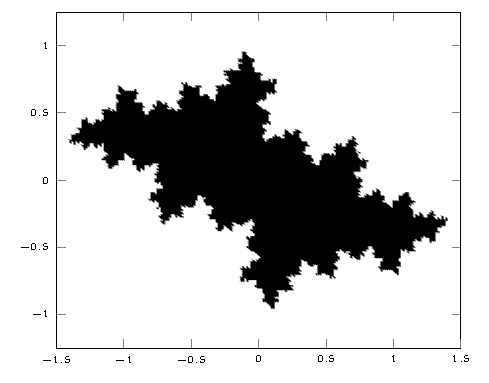
\includegraphics[scale=1]{img/img03_01_julia.pdf}
\caption{\textbf{Conjunt de presoners per a $c = -0.5 + 0.5i$.}
El conjunt de presoners per a $z \rightarrow z^{2} + c$, $c = -0.5 + 0.5i$ es mostra en negre. Els punts exteriors escapen a l'infinit.}
\label{fig13.15}
\end{figure}
\newpage
\section{Conjunt de Mandelbrot}
El conjunt de Mandelbrot és sens dubte el fractal més popular, probablement l'objecte més popular de les matemàtiques contemporànies. Algunes persones afirmen que no sols és l'objecte més bell sinó també el més complex que s'ha vist, és a dir, que s'ha fet visible. Des que Mandelbrot va realitzar el seu extraordinari experiment en 1979, ha estat duplicat per desenes de milers de científics aficionats de tot el món. A tots ells els agrada endinsar-se en la il·limitada varietat d'imatges que poden desenvolupar-se en la pantalla d'un ordinador. A vegades es necessiten moltes hores per a generar-les; però aquest és el preu que cal pagar per l'aventura de trobar una cosa nova i fantàstic on ningú ha mirat abans.

Aquesta riquesa és només un regal generós de les matemàtiques als qui els agrada meravellar-se amb les boniques imatges, o aquesta aparent bellesa i complexitat tenen un significat més profund? Les aparents característiques pictòriques del conjunt de Mandelbrot tenen una contrapartida igual en la seva bellesa matemàtica? En altres paraules, el conjunt de Mandelbrot presenta una visió del que els matemàtics de vegades anomenen l'estètica de les matemàtiques? La resposta és un ''sí'' vigorós.

\begin{figure}[!ht]
\centering
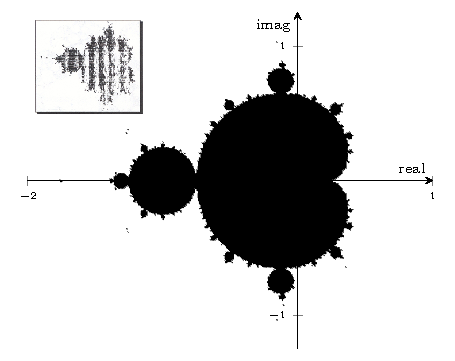
\includegraphics[scale=1]{img/06_mandelbrot_original.pdf}
\caption{\textbf{El conjunto de Mandelbrot - vella i nova representació.} La inserció mostra una impressió original de l'experiment de Mandelbrot.}
\label{fig06_mandelbrot_original}
\end{figure}

El conjunt de Mandelbrot s'obte de la següent funció:
\begin{align}\label{eq02_mandelbrot}
f(z)=z^2 + c,\quad z, c \in \mathbb{C}.
\end{align}
Primer es fixa un nombre complex \(c\) qualsevol. A partir de \(c\), es construeix una successió recursiva:
\begin{align*}
\left\{ \begin{array}{ll}
z_0 = 0,\quad & \text{termini inicial} \\
z_{n+1} = z_{n}^{2} + c,\quad & \text{successió recursiva.}
\end{array}\right.
\end{align*}
En general, els punts \(c\) pertanyen al subconjunt del pla complex  \([-2,2]\times[-2,2]\).

\subsection{Observem dos exemples}
Primer implementem en Python una funció denominada \textbf{successio\_c}, la qual crearà una successió d'un nombre complex arbitrari $c$.
{\setstretch{1.0}
\lstinputlisting{code/code03_01.py}}
\begin{eje}\label{eje2_1}
Prendre $c=-0.5 + 0.5i$
\end{eje}
{\setstretch{1.0}
\lstinputlisting{code/code03_02.py}}
Aquesta funció retorna un conjunt de dades amb les següents columnes:
\begin{itemize}
\item $c[k]$: índex de cadascun dels elements de la successió
\item succesió\_$c[k]$: elements de la successió del nombre complex $c$
\item mòdul\_$c[k]$: mòdul de cadascun dels elements de la successió
\end{itemize} 

\begin{table}[!ht]
\centering
{\UseRawInputEncoding
\begin{tabular}{lrr}
\toprule
  c[k] &  successi�\_c[k] &  m�dul\_c[k] \\
\midrule
  c[0] & -0.5000+0.5000$i$ &      0.7071 \\
  c[1] & -0.5000+0.0000$i$ &      0.5000 \\
  c[2] & -0.2500+0.5000$i$ &      0.5590 \\
  c[3] & -0.6875+0.2500$i$ &      0.7315 \\
  c[4] & -0.0898+0.1562$i$ &      0.1802 \\
  c[5] & -0.5163+0.4719$i$ &      0.6995 \\
  c[6] & -0.4561+0.0127$i$ &      0.4563 \\
  c[7] & -0.2921+0.4885$i$ &      0.5692 \\
  c[8] & -0.6533+0.2146$i$ &      0.6876 \\
  c[9] & -0.1193+0.2196$i$ &      0.2499 \\
 c[10] & -0.5340+0.4476$i$ &      0.6968 \\
 c[11] & -0.4152+0.0220$i$ &      0.4158 \\
 c[12] & -0.3281+0.4817$i$ &      0.5829 \\
 c[13] & -0.6244+0.1839$i$ &      0.6509 \\
 c[14] & -0.1439+0.2704$i$ &      0.3063 \\
 c[15] & -0.5524+0.4222$i$ &      0.6953 \\
 c[16] & -0.3731+0.0336$i$ &      0.3746 \\
 c[17] & -0.3619+0.4749$i$ &      0.5971 \\
 c[18] & -0.5946+0.1562$i$ &      0.6148 \\
 c[19] & -0.1709+0.3142$i$ &      0.3577 \\
\bottomrule
\end{tabular}
%\caption{Taula amb la successi� del nombre complex -0.5+0.5$i$ i els seus respectius m�duls. Es pot veure que en 19 iteracions tots aquests m�dul s�n menors que dos.}
}
\caption{Taula amb la successió del nombre complex -0.5+0.5$i$ i els seus respectius mòduls. Es pot veure que en 19 iteracions tots aquests mòduls són menors que dos.}
\label{tab03_04}
\end{table}
En la Taula \ref{tab03_04} es pot veure que en 19 iteracions el mòdul de tots els nombres $c[k]$, $k=0,\ldots,8$ és menor que dos. És a dir, $|c[k]|<2$ per a tot $k=0,\ldots,19$.
\begin{eje}\label{eje2_2}
Prendre $c= 0.5 + 0.5i$
\end{eje}
{\setstretch{1.0}
\lstinputlisting{code/code03_03.py}}
\begin{table}[!ht]
\centering
{\UseRawInputEncoding
\begin{tabular}{lrr}
\toprule
 c[k] &            successi�\_c[k] &   m�dul\_c[k] \\
\midrule
 c[0] &                0.50+0.50$i$ &         0.71 \\
 c[1] &                0.50+1.00$i$ &         1.12 \\
 c[2] &               -0.25+1.50$i$ &         1.52 \\
 c[3] &               -1.69-0.25$i$ &         1.71 \\
 c[4] &                3.29+1.34$i$ &         3.55 \\
 c[5] &                9.49+9.33$i$ &        13.30 \\
 c[6] &              3.47+177.50$i$ &       177.53 \\
 c[7] &        -31493.03+1231.54$i$ &     31517.10 \\
 c[8] & 990294278.68-77569977.40$i$ & 993327669.89 \\
\bottomrule
\end{tabular}
%\caption{Taula amb la successi� del nombre complex 0.5+0.5$i$ i els seus respectius m�duls. Es pot ser que a partir de la iteraci� 4 els m�duls s�n ma$i$ors que dos.}
}
\caption{Taula amb la successió del nombre complex 0.5+0.5$i$ i els seus respectius mòduls. Es pot ser que a partir de la iteració 4 els mòduls són majors que dos.}
\label{tab03_05}
\end{table}
Per contra, en Exemple \ref{eje2_2} es pot veure que en 8 iteracions a partir del nombre $c[4]$, el mòdul és major que dos. És a dir, $|c[k]|>2$, per a $k=4,\ldots,8$.

Mandelbrot va establir que tots els punts $c$ que compleixin amb la condició de l'Exemple \ref{eje2_1} per a un cert nombre màxim d'iteracions (per a aquest estudi s'ha establert en 9, però pot ser qualsevol, per exemple: 15, 20, 50, etc.) es pinten de color negre. Cas contrari, punts com l'Exemple \ref{eje2_2}, es pinten de color blanc (veure Figura \ref{fig06_mandelbrot_bw}).

\begin{figure}[!ht]
\centering
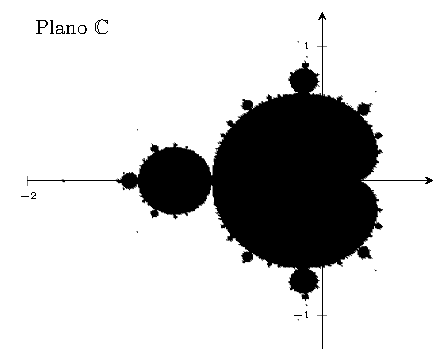
\includegraphics[width=0.5\textwidth]{img/07_mandelbrot_bw}
\caption{Conjunt de Mandelbrot.}
\label{fig06_mandelbrot_bw}
\end{figure}

\subsection{Matriu d'iteracions}
El nostre objectiu és crear una matriu que mostri el nombre d'iteracions d'un conjunt de nombres complexos $c$ que s'obtenen de la funció $f(z)=z^{2}+c$, amb $z=0$.
\paragraph*{Obtenir la iteració $k$.} Crear una funció que retorni la iteració $k$ on el mòdul del nombre complex $c$ és major que dos.
{\setstretch{1.0}
\lstinputlisting{code/code03_04.py}}

\paragraph*{Taula amb diferents nombres complexos $c$.} Farem una reixeta amb 81 nombres complexos en l'interval 2D $[-2,2]\times[-2,2]$ amb un espaiat de 0.5.
{\setstretch{1.0}
\lstinputlisting{code/code03_05.py}}

\begin{table}[!ht]
{\UseRawInputEncoding
\resizebox{\textwidth}{!}{
\begin{tabular}{lccccccccc}
\toprule
{} &            0 &            1 &            2 &            3 &           4 &           5 &           6 &           7 &           8 \\
\midrule
0 &  -2.0-2.0$i$ &  -2.0-1.5$i$ &  -2.0-1.0$i$ &  -2.0-0.5$i$ &  -2.0+0.0$i$ &  -2.0+0.5$i$ &  -2.0+1.0$i$ &  -2.0+1.5$i$ &  -2.0+2.0$i$ \\
1 &  -1.5-2.0$i$ &  -1.5-1.5$i$ &  -1.5-1.0$i$ &  -1.5-0.5$i$ &  -1.5+0.0$i$ &  -1.5+0.5$i$ &  -1.5+1.0$i$ &  -1.5+1.5$i$ &  -1.5+2.0$i$ \\
2 &  -1.0-2.0$i$ &  -1.0-1.5$i$ &  -1.0-1.0$i$ &  -1.0-0.5$i$ &  -1.0+0.0$i$ &  -1.0+0.5$i$ &  -1.0+1.0$i$ &  -1.0+1.5$i$ &  -1.0+2.0$i$ \\
3 &  -0.5-2.0$i$ &  -0.5-1.5$i$ &  -0.5-1.0$i$ &  -0.5-0.5$i$ &  -0.5+0.0$i$ &  -0.5+0.5$i$ &  -0.5+1.0$i$ &  -0.5+1.5$i$ &  -0.5+2.0$i$ \\
4 &   0.0-2.0$i$ &   0.0-1.5$i$ &   0.0-1.0$i$ &   0.0-0.5$i$ &   0.0+0.0$i$ &   0.0+0.5$i$ &   0.0+1.0$i$ &   0.0+1.5$i$ &   0.0+2.0$i$ \\
5 &   0.5-2.0$i$ &   0.5-1.5$i$ &   0.5-1.0$i$ &   0.5-0.5$i$ &   0.5+0.0$i$ &   0.5+0.5$i$ &   0.5+1.0$i$ &   0.5+1.5$i$ &   0.5+2.0$i$ \\
6 &   1.0-2.0$i$ &   1.0-1.5$i$ &   1.0-1.0$i$ &   1.0-0.5$i$ &   1.0+0.0$i$ &   1.0+0.5$i$ &   1.0+1.0$i$ &   1.0+1.5$i$ &   1.0+2.0$i$ \\
7 &   1.5-2.0$i$ &   1.5-1.5$i$ &   1.5-1.0$i$ &   1.5-0.5$i$ &   1.5+0.0$i$ &   1.5+0.5$i$ &   1.5+1.0$i$ &   1.5+1.5$i$ &   1.5+2.0$i$ \\
8 &   2.0-2.0$i$ &   2.0-1.5$i$ &   2.0-1.0$i$ &   2.0-0.5$i$ &   2.0+0.0$i$ &   2.0+0.5$i$ &   2.0+1.0$i$ &   2.0+1.5$i$ &   2.0+2.0$i$ \\
\bottomrule
\end{tabular}
}
%\caption{Taula amb els 81 nombres complexos}
}
\caption{Taula amb els 81 nombres complexos}
\label{tab03_06}
\end{table}

En la fila 3 i columna 5 de la Taula \ref{tab03_06} es pot veure el nombre complex $ -0.5 + 0.5i$ (veure Exemple \ref{eje2_1}). Per a aquest número en 19 iteracions el mòdul de tots els seus elements eren menors que 2. Per tant, assignem amb un 19 a aquesta cel·la. D'altra banda, en la fila 5 i columna 5 es pot veure el nombre complex $ 0.5 + 0.5i$ (veure Exemple \ref{eje2_2}), per a aquest nombre a partir de la iteració 4 el mòdul de tots els seus elements eren majors que 2. Per tant, assignem amb un 4 a aquesta cel·la.

\paragraph*{Visualitzar la matriu d’iteracions.} Imprimir una matriu amb el nombre d'iteracions que compleix amb la condició mòdul major que 2 per a cadascun dels 81 nombres complexos.
{\setstretch{1.0}
\lstinputlisting{code/code03_05_01.py}}
\begin{table}[!ht]
\centering
{\UseRawInputEncoding
\begin{tabular}{lrrrrrrrrr}
\toprule
{} &  0 &  1 &  2 &  3 &  4 &  5 &  6 &  7 &  8 \\
\midrule
0 &  0 &  0 &  0 &  0 & 19 &  0 &  0 &  0 &  0 \\
1 &  0 &  0 &  1 &  2 & 19 &  2 &  1 &  0 &  0 \\
2 &  0 &  1 &  2 &  4 & 19 &  4 &  2 &  1 &  0 \\
3 &  0 &  1 &  3 & 19 & 19 & 19 &  3 &  1 &  0 \\
4 &  1 &  1 & 19 & 19 & 19 & 19 & 19 &  1 &  1 \\
5 &  0 &  1 &  1 &  4 &  4 &  4 &  1 &  1 &  0 \\
6 &  0 &  1 &  1 &  1 &  2 &  1 &  1 &  1 &  0 \\
7 &  0 &  0 &  1 &  1 &  1 &  1 &  1 &  0 &  0 \\
8 &  0 &  0 &  0 &  0 &  1 &  0 &  0 &  0 &  0 \\
\bottomrule
\end{tabular}
%\caption{Matriu d'iterations}
}
\caption{Matriu d'iterations}
\end{table}

\paragraph*{ Dibuixar la matriu d'iteracions.}\hspace*{0px}
{\setstretch{1.0}
\lstinputlisting{code/code03_06.py}}

\begin{figure}[!ht]
\centering
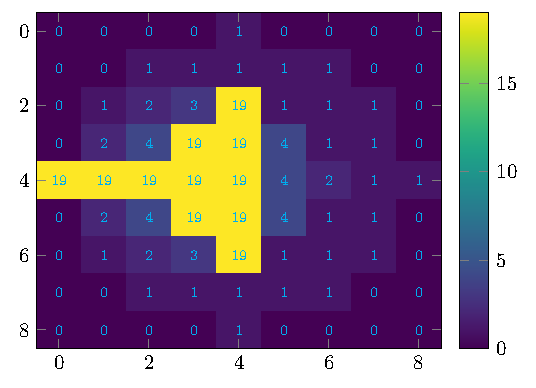
\includegraphics[scale=1.4]{img/matrix_mandelbrot.pdf}
\caption{\textbf{Gràfic de la matriu d'iteracions.} La barra de colors indica el nombre d'iteracions d'un nombre complex fins que es dispara de 0 (morat) a 19 (groc). A la figura s'indica el nombre d'iteracions que té cada nombre complex de la Taula \ref{tab03_06}.}
\end{figure}

\begin{figure}[!ht]
\centering
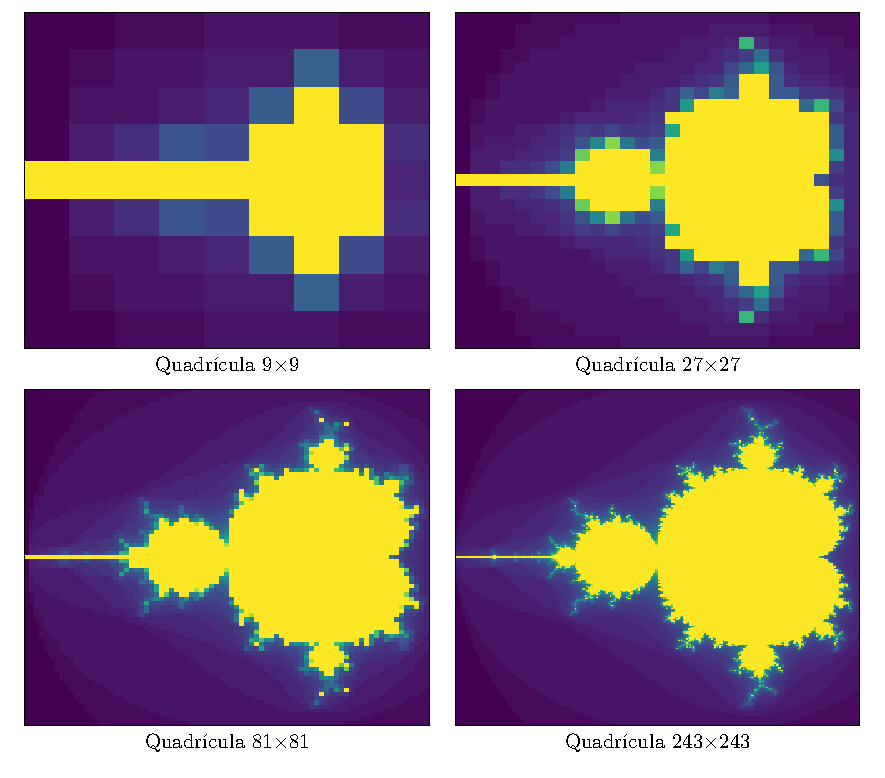
\includegraphics[scale=1]{img/several_mandelbrot.pdf}
\caption{\textbf{4 conjunts de Mandelbrot.}  Cadascun amb un conjunt de punts major.}
\end{figure}

\chapter{CARACTERÍSTIQUES DELS FRACTALS}
\section{Característiques generals}
En ser figures tan diferents de les tradicionals formes euclidianes, els fractals presenten característiques úniques:
\begin{itemize}
\item Són formes recursives
\item Presenten autosimilitud
\item No tenen dimensió amb valor natural, sinó irracional
\end{itemize}
També, tenen la qualitat de ser figures amb superfície finita, però perímetre infinit, això, pel fet que són figures que es repeteixen a diferents escales.
\section{Autosimilitud}
El concepte d'autosimilitud o autosemblança és una propietat dels fractals el qual consisteix en el fet que tot un conjunt és igual o semblant en totes les parts de si mateix, de tal manera que el cos es pot engrandir o encongir i encara seguirà sent igual. Un exemple de la natura d’autosimilitud són les ones del mar. 

Matemàticament, l’autosimilitud és un terme amb diferents conceptes o tipus d’autosimilitud. Aquests tipus d’autosimilitud presenten diferències entre si mateixos, però, comparteixen la característica tenir semblança a escala.
\begin{figure}[!ht]
\centering
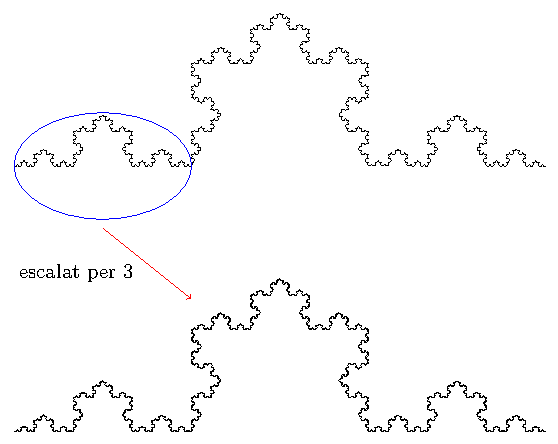
\includegraphics[scale=1]{img/img02_01_kock.pdf}
\caption{\textbf{Ampliació de la corba de Koch.} Un quart de la corba de Koch (a dalt) es magnifica per un factor de 3. A causa de l'autosimilitud de la corba de Koch, el resultat és una còpia de la corba completa.}
\end{figure}
\subsection{Autosimilitud exacta}
Es diu que hi ha autosimilitud exacta quan una o diverses parts d'un tot repeteixen exactament la seva similitud amb aquest tot. L'autosimilitud exacta permet l'amplificació successiva amb repetició exacta única, múltiple o infinita de les propietats inicials. %L'autosimilitud exacta apareix a vegades en sistemes de funcions iterades (IFS).
\subsection{Autosimilitud aproximada}
L'autosimilitud aproximada o quasi-autosimilitud es troba sovint en la naturalesa (autosimilitud natural). Es caracteritza per no condensar la propietat d'autosimilitud en  tot el conjunt, és a dir, hi existeixen petites diferències entre la part i el tot.
\begin{figure}[!ht]
\centering
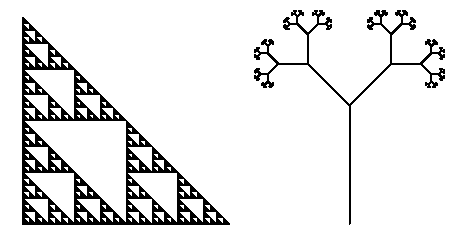
\includegraphics[scale=1]{img/img02_02_TreeSierpinski.pdf}
\caption{\textbf{Dues diferents estructures autosemblants} La junta de Sierpiński (esquerra) és autosemblant en tots els seus punts, mentre que l'arbre de dues branques (dreta) és semblant només en les fulles.}
\end{figure}
\subsection{Autosimilitud estadística}
L'autosimilitud estadística és la menys exigent. Només es conserven algunes propietats estadístiques durant el canvi d'escala, com a les muntanyes o en els cràters lunars.
\section{Dimensions fraccionàries o fractals}
Tota figura geomètrica o cos que es pugui representar al pla, per norma general, té el que anomenem dimensions. Per exemple una recta té una dimensió, un quadrat dos i un cub tres. Això és el que s’anomena dimensió topogràfica. Aquesta dimensió topogràfica, normalment, és un nombre natural (1, 2 i 3). Tot i això, aquesta norma no hi aplica pels fractals, els quals, tenen una dimensió topològica amb nombre irracional, aquesta característica va donar lloc a què molts matemàtics intentessin determinar on tenen cabuda els fractals, respecte al camp de les dimensions, és aquí on apareix el terme dimensió fractal o fraccionària. La dimensió fractal es va idear amb l’objectiu d’analitzar la dimensió irracional dels fractals en el pla, amb el temps, es van donar diverses definicions i es van elaborar diferents dimensions per aquesta, com poden ser la dimensió de Hausdorff-Besicovitch, dimensió de comptatge de caixes, dimensió d'euclidiana, dimensió de capacitat, dimensió d’informació, etc. Hi existeixen moltes, i totes estan relacionades, però no totes tenen la mateixa importància. De totes aquestes, destaquen la dimensió d'autosimilitud i la de comptatge de caixes.
\subsection{Dimensió d'autosimilitud}
Per a definir la dimensió d'autosimilitud \cite[p.~194]{FistCourseChaos}, primer analitzarem alguns cossos autosimilars trivials (una línia, un quadrat i un cub) de la següent manera:

\begin{figure}[!ht]
\centering
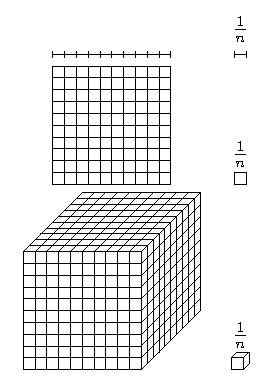
\includegraphics[scale=1.5]{img/img02_dim_auto.pdf}
\caption{Il·lustrant el nombre de còpies petites d'un objecte que caben dins d'una còpia gran.}
\label{img02_01}
\end{figure}
Una línia de longitud 1 és un objecte molt autosimilar: Pot dividir-se en $n = n^1$ petites peces, cadascuna de les quals és exactament $\displaystyle\frac{1}{n}$ de la grandària de la línia original i cadascuna de les quals, quan s'amplia per un factor $n$, s'assembla exactament a la línia original (veure Figura \ref{img02_01}).

Per a un quadrat de costat 1, si el dividim en quadrats de costat $\displaystyle\frac{1}{n}$ de l'original obtindrem $n\times n$ quadrats petits. Per tant, es requereix $n^2$ quadrats petits per obtenir l'original.

En el cas d'un cub de costat 1, en dividir-ho per peces de costat $\displaystyle\frac{1}{n}$, s'obtindran $n^3$ peces més petites, les necessàries per reconstruir el cub original.

\begin{table}[!ht]
\centering
{\UseRawInputEncoding
\begin{tabular}{|l|c|c|} 
\hline
& & Nombre de copies petites que \\
Coss & Factor d'augment & caben en una copia gran \\
\hline 
L��nia & 3 & $3=3^1$ \\
Quadrat & 3 & $9=3^2$ \\
Cub & 3 & $27=3^3$ \\
\hline
\end{tabular}


}
\caption{Efectes de l'ampliació en diferents cossos.}
\label{tab02_01}
\end{table}
En aquests 3 casos, l'exponent distingeix la dimensió de l'objecte en qüestió. En la taula \ref{tab02_01} hem pres $n$=3 per a dividir la línia, el quadrat i el cub, en la tercera columna podem veure que cadascun dels exponents estan relacionats amb la dimensió dels cossos anteriors. A més, la base 3 representa el factor d'augment. Per tant, obtenim la següent igualtat.
\begin{align}
\text{nombre de còpies petites} = (\text {factor d'augment})^{D},
\label{eq02_01}
\end{align}
on $D$ és la dimensió. Finalment, aplicant logaritme a banda i banda de la igualtat \ref{eq02_01} obtenim
\begin{align}
D = \frac{\log(k)}{\log(M)} = \frac{\log(\text{nombre de còpies petites})}{\log(\text{factor d'augment})}.
\label{eq02_02}
\end{align}

\begin{eje}
\label{eje03_dim_auto}
Trobar la dimensió del triangle de Sierpiński amb el mètode d'autosimilitud.
\end{eje}
\begin{myproof}
Per al triangle de Sierpiński, recordem que podem subdividir aquesta figura en tres peces autosimilars, cadascun dels quals pot ampliar-se per un factor de 2 per a obtenir la figura completa. Així, tenim
\begin{align*}
D = \frac{\log(k)}{\log(M)} = \frac{\log(\text{nombre de triangles})}{\log(\text{factor d'augment})}=\frac{\log 3}{\log 2}=1.584962501,
\end{align*}
el qual no és en absolut un nombre enter! Provem de nou. El triangle de Sierpiński també es pot construir muntant nou peces més petites. Cadascuna d'aquestes peces més petites és exactament una quarta part de la mida de la figura original. Per tant,
\begin{align*}
D = \frac{\log 9}{\log 4} = \frac{\log 3^2}{\log 2^4} = \frac{2\log 3}{2\log 2}=\frac{\log 3}{\log 2}=1.584962501,
\end{align*}
i tenim la mateixa dimensió.
\end{myproof}
\subsection{Dimensió de comptatge de caixes/Haussdorff}
%Definición de la dimensión de recuento de cajas
La dimensió de comptatge de caixes o de Haussdorff \cite[p.~93]{KitchenScience}, és una de les tantes nocions, respecte a la dimensió fractal, aquesta destaca per ser un la més eficient en aplicacions científiques. Aquesta noció de dimensió fractal empra quadrícules, que denominarem caixes, les quals són superposades a una forma fractal. En fer això, es fa un recompte del nombre de caixes ($N(r)$), de mesura $r$, necessàries per a cobrir una forma. Però, com depèn $N(r)$ de $r$? Per a respondre aquesta pregunta, observem com es comporta aquesta relació en 1, 2 i 3 dimensions (veure Figura \ref{img02_01_box}).

\begin{figure}[!ht]
\centering
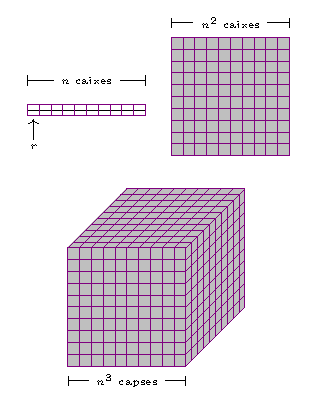
\includegraphics[scale=1.5]{img/img02_dim_box.pdf}
\caption{La línia, el quadrat i el  cub, tots de costat 1. En tots els casos les  caixes que els cobreixen tenen els seus costats com mesurada $\displaystyle r=\frac{1}{n}$.}
\label{img02_01_box}
\end{figure}

\begin{itemize}
\item Si la forma és unidimensional, com el segment de recta, veiem que $N(r) = \displaystyle\frac{1}{r}$.
\item Si la forma és bidimensional, com el quadrat unitari (omplert), veiem que $N(r) = \displaystyle\left(\frac{1}{r}\right)^2$
\item Si la forma és tridimensional, com el cub unitari (omplert), veiem que $N(r) = \displaystyle\left(\frac{1}{r}\right)^3$.
\end{itemize}
Per a formes més complexes, la relació entre $N(r)$ i $\displaystyle\frac{1}{r}$ pot no ser tan clara. Si suposem que $N(r)$ és aproximadament $k\displaystyle\left(\frac{1}{r}\right)^d$, una relació de llei de potència, com podem trobar $d$?

Prenent el logaritme de tots dos costats de $N(r) = k\displaystyle\left(\frac{1}{r}\right)^d$ , obtenim:
\begin{align*}
 \log(N(r))  &= \log(k) + \log\left(\frac{1}{r}\right)^d \\
             &= \log(k) + d\log\left(\frac{1}{r}\right).  
\end{align*}
Amb l'expectativa que l'aproximació es fa millor per a $r$ més petit. Resolent per a $d$ i prenent el límit quan $r \rightarrow 0$, tenim:
\begin{align*}
 d = \lim_{r\rightarrow 0}\frac{\log(N(r))}{\log(\frac{1}{r})} 
\end{align*}
Observi que quan $r\rightarrow 0$ tenim $\displaystyle\frac{1}{r}\rightarrow \infty$, llavors $\displaystyle\log\left(\frac{1}{r}\right)\rightarrow \infty$ i $\displaystyle\frac{\log(k)}{\log(\frac{1}{r})} \rightarrow 0$.

Si el límit existeix, es denomina dimensió de comptatge de caixes, $d$, de la forma. Aquest límit pot ser lent per a convergir; un enfocament alternatiu és observar que
\begin{align*}
\log(N(r))  = \log(k) + d\log\left(\frac{1}{r}\right), 
\end{align*}
és l'equació d'una recta amb pendent $d$ i intercepció$-y$, $\log(k)$. Per tant, si representem $\log(N(r))$ enfront de $\displaystyle\log\left(\frac{1}{r}\right)$, els punts haurien de situar-se aproximadament en una línia recta amb pendent $d$. Aquest és el mètode $log-log$ per a trobar la dimensió de comptatge de caixes.

\begin{eje}
Trobar la dimensió del triangle de Sierpiński amb el mètode de comptatge per caixes.
\end{eje}
\begin{myproof}
Per a aquest exemple  utilitzarem  4 quadrícules  amb caixes de costat $r_1=\displaystyle\frac{1}{8}$, $r_2=\displaystyle\frac{1}{16}$,  $r_3=\displaystyle\frac{1}{32}$ i $r_4=\displaystyle\frac{1}{64}$. Després, per a cada quadrícule,  comptarem el nombre de caixes que cobreixen el triangle de Sierpiński (vegeu Taula \ref{tab03_00_box}). Finalment, trobem els 4 punts $\left(\log\left(\displaystyle\frac{1}{r}\right),\log(N(r))\right)$ en el pla, els quals seran necessaris per a obtenir la recta que millor s'ajusta a aquests 4 punts. 

Per tant, la dimensió de comptatge de caixes del triangle de Sierpinński és el pendent de la recta $y = 1.584963x$ (veure Figura \ref{img03_dim_box}), que és  el mateix resultat que es va obtenir en l'Exemple \ref{eje03_dim_auto}.

\begin{figure}[!ht]
\centering
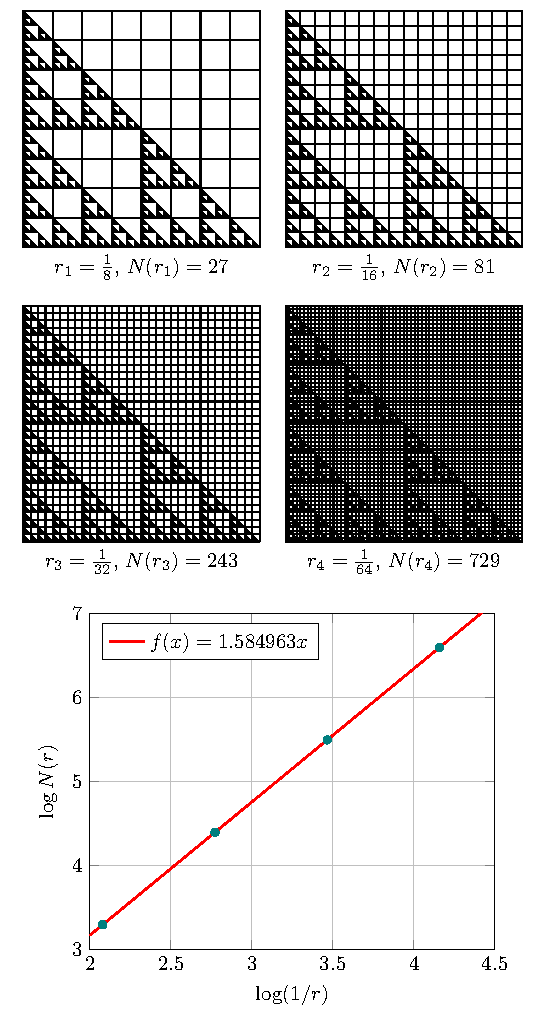
\includegraphics[width=0.5\textwidth]{img/img02_dim_sierpinski.pdf} 
\caption{\textbf{Triangle de Sierpinński.} Comptatge de caixes utilitzant 4 quadrícules, el pendent de la recta que s'ajusta als 4 punts és 1.584963.}
\label{img03_dim_box}
\end{figure}
\begin{table}[!ht]
\centering
{\UseRawInputEncoding
%\begin{tabular}{ccc}
%\toprule
%$r$ & $N(r)$ & $\left(\log(\displaystyle\frac{1}{r}),\log(N(r))\right)$ \\
%\midrule
%$\displaystyle\frac{1}{8}$  & 27  &(2.0794, 3.2958)\\
%$\displaystyle\frac{1}{16}$ & 81  &(2.7726, 4.3944)\\
%$\displaystyle\frac{1}{32}$ & 243 &(3.4657, 5.4931)\\
%$\displaystyle\frac{1}{64}$ & 729 &(4.1589, 6.5917)\\
%\bottomrule
%\end{tabular}
%\renewcommand{\arraystretch}{2.75}
{\tabulinesep=1.5mm
\begin{tabu}{|l|cccc|}
\hline
$r$ & $\displaystyle\frac{1}{8}$ & $\displaystyle\frac{1}{16}$ & $\displaystyle\frac{1}{32}$ & $\displaystyle\frac{1}{64}$\\
\hline
$N(r)$ & 27 & 81 & 243 & 729 \\
\hline
$\log\left(\displaystyle\frac{1}{r}\right)$ & 2.0794 & 2.7726 & 3.4657 & 4.1589\\
\hline
$\log(N(r))$ & 3.2958 & 4.3944 & 5.4931 & 6.5917\\
\hline
\end{tabu}}
}
\caption{4 quadrícules del triangle de Sierpiński amb caixes de costat $r_1=1/8$, $r_2=1/16$,  $r_3=1/32$ i $r_4=1/64$.}
\label{tab03_00_box}
\end{table}
\end{myproof}
\newpage
\begin{eje}
Trobar la dimensió del contorn del mapa d'Espanya amb el mètode de comptatge de caixes.
\end{eje}
\begin{myproof}
Per a aquest exemple  utilitzarem  3 quadrícules  amb caixes de costat $r_1=\displaystyle\frac{1}{6}$, $r_2=\displaystyle\frac{1}{12}$ i  $r_3=\displaystyle\frac{1}{24}$. Després, per a cada quadrícula, comptarem el nombre de caixes que cobreixen el mapa d'Espanya que són $N(r_1)=23$, $N(r_2)=52$ i $N(r_3)=121$ respectivament (veure Figura \ref{img03_dim_country}). 

\begin{figure}[!ht]
\centering
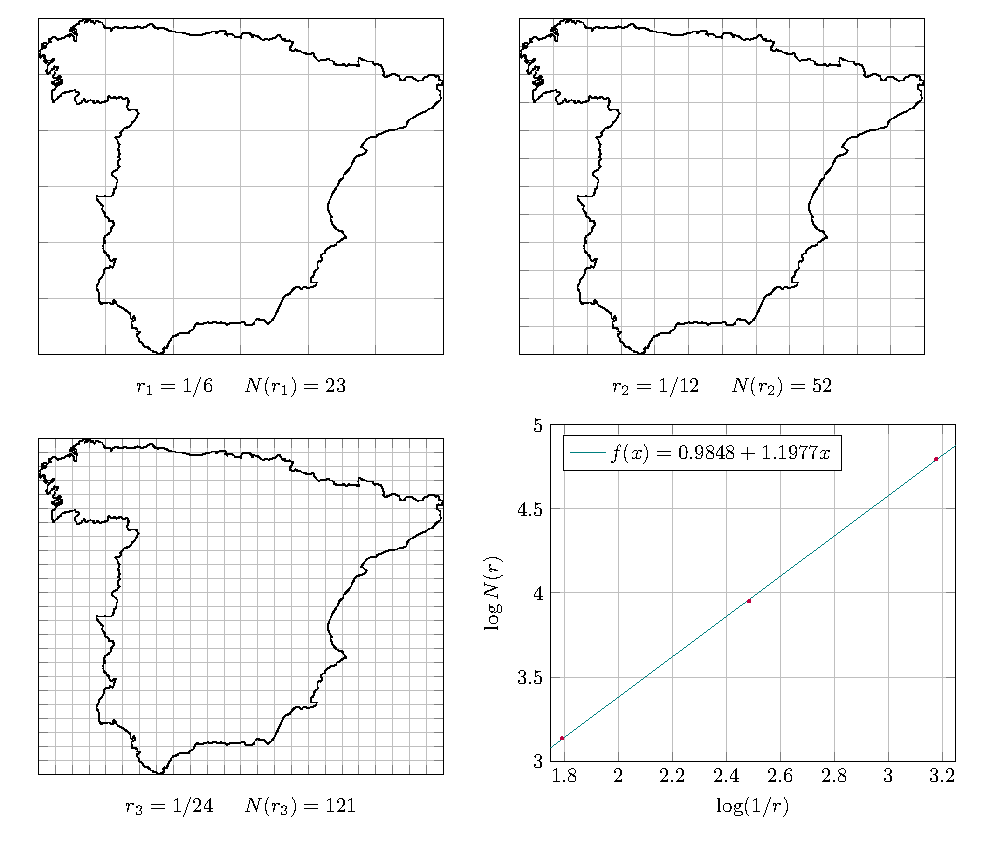
\includegraphics[width=.75\textwidth]{img/img02_dim_country.pdf} 
\caption{Comptatge de caixa utilitzant 3 quadrícules, el pendent de la recta que s'ajusta als 3 punts és 1.1977.}
\label{img03_dim_country}
\end{figure}
\end{myproof}
\newpage
Actualment, gràcies als avanços en informàtica, podem deixar de costat aquest mètode tan rudimentari, però funcional, i usar mesures $r$ més petites per a aproximar-nos cada vegada més al valor real de la dimensió fractal de qualsevol forma. 

\begin{small}
\UseRawInputEncoding
\begin{longtable}[c]{|c|c|c|c|}
\caption{Dimensi� dels fractals estudiats en aquest treball.}\\
\hline
\textbf{Valor real} & \textbf{Valor aproximat} & \textbf{Nom} & \textbf{Representaci�} \\
\hline
\endfirsthead
\multicolumn{4}{c}%
{\tablename\ \thetable\ -- \textit{Continua de la p�gina anterior}} \\
\hline
\textbf{Valor real} & \textbf{Valor aproximat} & \textbf{Nom} & \textbf{Representaci�} \\
\hline
\endhead
\hline \multicolumn{4}{r}{\textit{Continua en la p�gina seg�ent}} \\
\endfoot
\hline
\endlastfoot
\hline
$\frac{\log(2)}{\log(3)}$ & 0.6309 & conjunt de Cantor & 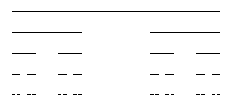
\includegraphics[width=3.75cm, valign = c]{img/img02_03_cantor.pdf}\\
\hline
$\frac{\log(4)}{\log(3)}$ & 1.2619 & corba de Koch & 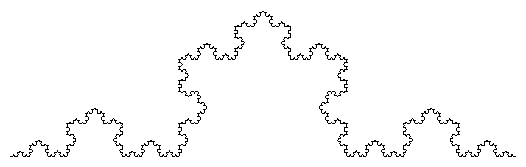
\includegraphics[width=3.75cm, valign = c]{img/img02_04_koch.pdf}\\
\hline
$\frac{\log(3)}{\log(2)}$ & 1.585 & triangle de Sierpi\'{n}ski & 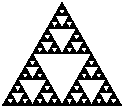
\includegraphics[width=3.75cm, valign = c]{img/img02_05_sierpinski.pdf}\\
\hline
$\frac{\log(2)}{\log(3)}$ & 1.8928 & catifa de Sierpi\'{n}ski & 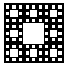
\includegraphics[width=3.75cm, valign = c]{img/img02_06_carpet.pdf}\\
\hline
$\frac{\log(2)}{\log(\sqrt{2})}$ & 2 & corba de drac & 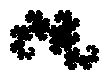
\includegraphics[width=3.75cm, valign = c]{img/img03_dragon_curve.pdf}\\
\hline
$\frac{\log(4)}{\log(2)}$ & 2 & tetraedre de Sierpi\'{n}ski & 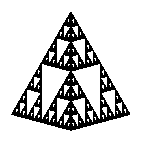
\includegraphics[width=3.75cm, valign = c]{img/img02_08_tetraedro.pdf}\\
\hline
$\frac{\log(20)}{\log(3)}$ & 2,7268 & esponja de Menger & 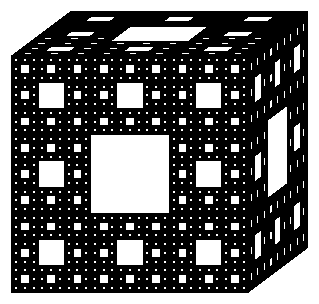
\includegraphics[width=3.75cm, valign = c]{img/img02_09_menger.pdf}\\
\hline
2 & 2 & corba de Peano & 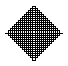
\includegraphics[width=3.75cm, valign = c]{img/img02_10_peano.pdf}\\
\hline
2 & 2 & conjunt de Julia & \includegraphics[width=3.75cm, valign = c]{img/img03_01_julia.pdf}\\
\hline
2 & 2 & conjunt de Mandelbrot & \includegraphics[width=3.75cm, valign = c]{img/img02_12_mandelbrot.pdf}\\
\hline
\end{longtable}

\end{small}
\section{Recursivitat}
L'última característica important dels fractals és la seva recursivitat. La recursivitat es defineix com la propietat d'una unitat o procés de construir-se mitjançant la repetició de si mateix indefinidament.

\chapter{FRACTALS A LA NATURA}\label{fractals_nature}
\section{Geometria de la natura}
Com vam mencionar en apartats anteriors, les formes fractals són la geometria de la naturalesa, és a dir, la geometria fractal es pot trobar en la natura, en moltes parts i amb diverses formes.  

La manera més comuna en la qual podem trobar els fractals a la natura són els paisatges i elements de la natura \cite{FractalWorlds}, els quals, presenten una forma que escapa de la concepció ''perfecta'' de la geometria euclidiana, ja que presenten autosimilitud, però, d'una manera no tan exacta, és a dir, els elements naturals amb forma fractal presenten quasi similitud.
\subsection{Rius}
Les xarxes o formacions d'aigua com rius són altre exemple de la fractalitat del món. Els fractals són emprats en l'estudi dels rius de dues maneres.  El patró del rierol dels rius segueix una forma fractal, perquè un riu es divideix en corrents d'aigua més petites i així successivament. Aquest procés es repeteix en la riba de les conques on presenten límits fractals a diferents escales.
\begin{figure}[!ht]
\centering
\includegraphics[scale=1]{img/img04_dona.pdf}
\caption{\textbf{Doñana.} Fotografies fetes per Héctor Garrido al Parc de Doñana \cite{Miteco}. Rius i maresmes amb estructura fractal.}
\end{figure}

L'exemple de riu ''fractal'' seria un riu trenat. Un riu trenat o riu entrellaçat té un llit que consisteix en una xarxa de canals separats per bancs o petites illes. Aquestes formacions d'aigua presenten quasi similitud a diverses escales des dels punts més externs del riu fins al naixement d'aquest.

\begin{figure}[!ht]
\centering
\includegraphics[scale=0.7]{img/img04_02_braided.png}
\caption{\textbf{Riu entrellaçat.} Fotografia del riu Tasman a Nova Zelanda.}
\end{figure}
\newpage
\subsection{Raigs}
Els llamps presenten una estructura semblant a la d'un arbre fractal, ja que cada extensió d'aquest és una còpia d'una extensió inicial (iniciador). Per tant, cada extensió d'un raig és igual en tot el seu conjunt. La idea dels raigs com a fractals ve des de la concepció de les figures de Lichtenberg. Georg Christoph Lichtenberg va generar imatges produïdes descàrregues elèctriques ramificades sobre superfícies o interiors de materials aïllants, on es va observar que aquestes figueres presentaven ramificacions autosimilars. 
\begin{figure}[!ht]
\centering
\includegraphics[scale=1]{img/img04_rayos.pdf}
\caption{\textbf{Raigs.} A l'esquerra, imatges de 3 llamps diferents. A la dreta, una figura de Lichtenberg continguda en un vidre.}
\end{figure}
\subsection{Muntanyes}
Les muntanyes també presenten fractalitat en la seva estructura. Aquests accidents geogràfics, producte de les forces tectòniques i l'erosió de l'aigua, presenten en els seus pics i barris formacions més petites d'aquestes a diferents escales. Observant, la propietat d'autosimilitud. La  fractalitat  de les muntanyes va ser estudiada per Sig Handelman, Richard Voss i Ken Musgrave, els qui eren col·legues de Mandelbrot. Ells van mesurar la rugositat de les muntanyes i després van utilitzar aquests valors en programes, obtenint falsificacions fractals realistes i complexes. Aquestes falsificacions van ser utilitzades per Mandelbrot en les seves classes sobre geometria fractal en  Yale, on les compara amb fotos de muntanyes reals, mostrant que només tenen lleugeres diferències. D'aquesta manera es va demostrar la naturalesa fractal de les muntanyes, perquè segueixen la mateixa ''aleatorietat'' per a formar-se.
\begin{figure}[!ht]
\centering
\includegraphics[scale=1]{img/img04_mountains.pdf}
\caption{\textbf{Muntanyes.} A l'esquerra, una muntanya feta per un programa mitjançant fractals. A la dreta, una muntanya dels Pirineus.}
\end{figure}
\section{La fractalitat dels éssers vius}
Els éssers vius també tenim certa naturalesa fractal \cite[p.~55]{FractalWorlds}. Les plantes presenten una estructura autosimilar en els seus raïms de flors i les seves arrels. El nostre interior també és una font d'estructures amb naturalesa fractal: sistema respiratori, circulatori i nervis. Els quals tenen models fractals.
\subsection{Els pulmons}
Els nostres pulmons són una estructura fractal per excel·lència. La finalitat dels pulmons és la de proporcionar oxigen pel nostre organisme, aquest òrgan té la capacitat de contenir mig litre d'aire i després intercanviar oxigen per $CO_{2}$ en menys d'un segon. Un procés tan exigent com aquest necessitaria una superfície gran, la qual, hauria d'estar continguda en un volum petit. Per fer-nos una idea, la superfície que ocupen els pulmons és de 130 $m^{2}$, mentre que els pulmons només poden contenir entre 5 a 6 litres d'oxigen. 

Per dur a terme aquest procés els pulmons disposen de la tràquea i de les 23 generacions de ramificacions de l'arbre bronquial sumat els alvèols. Aquest sistema resulta eficient, però aquesta eficiència es deu a la disposició de la seva estructura, la qual és autosimilar.  Les branques respiratòries es van dividint durant les 23 generacions en branques mare i filla. Aquestes estan dissenyades perquè en la zona d'intercanvi d'oxigen els seus diàmetres tinguin pocs canvis, alentint el flux d'aire.   
\begin{figure}[!ht]
\centering
\includegraphics[scale=1]{img/img04_lung.pdf}
\caption{\textbf{Pulmons.} A l'esquerra, un model dels pulmons. A la dreta, una imatge ampliada d'un pulmó.}
\end{figure}
\subsection{El sistema circulatori}
El sistema cardiovascular és un altre exemple de geometria fractal dins del cos. Les ramificacions del sistema circulatori (venes, artèries i capil·lars) tenen la missió de transportar sang per tot el cos.  De la mateixa manera que amb el sistema respiratori, el sistema circulatori presenta unes dimensions exorbitades en comparació amb el nostre cos. Si es posa tots els vasos sanguinis d'un cos humà en línia recta, s'assoliria una longitud de 96000 km, una cosa impossible de contenir en un cos humà. Llavors ''Com pot ser això?'', la resposta és la mateixa que amb el sistema respiratori, una estructura amb naturalesa fractal. Les ramificacions del sistema circulatori estan dissenyades per augmentar i disminuir-se a diferents escales, és a dir, presenta autosimilitud.

La presència dels fractals en el sistema circulatori també està present en el tractament de malalties coronàries. Molts estudis científics van demostrar que un cor malalt presenta una variació de la seva dimensió fractal, respecte a la d'un cor sa. Per fer-ho, s'utilitza el mètode de comptatge de capses, amb el qual, s'obté la dimensió fractal del cor. Un exemple, seria la malaltia de l'artèria oclusiva greu, on varia la dimensió fractal de l'arbre coronari esquerra.
\section{Altres formacions naturals fractals}
Existeixen moltes altres formacions naturals tant del medi ambient com dins nostre, que presenten la característica d'autosimilitud dels fractals. A continuació una taula amb més formacions fractals:
\begin{table}[!ht]
\centering
{\UseRawInputEncoding
{\tabulinesep=1.25mm
\begin{tabu}{|c|p{4cm}|}
\hline
Nom & Representaci�\\
\hline
Ull & \includegraphics[valign=c, width=3.75cm]{img/img04_06_ojo_humano.jpeg}\\
\hline
N�vols & \includegraphics[valign=c, width=3.75cm]{img/img04_06_nubes.jpeg}\\
\hline
ADN & \includegraphics[valign=c, width=3.75cm]{img/img04_06_glo.jpeg}\\
\hline
Falgueres & \includegraphics[valign=c, width=3.75cm]{img/img04_06_helechos.jpeg}\\
\hline
Romanesco & \includegraphics[valign=c, width=3.75cm]{img/img04_06_brocoli.jpeg}\\
\hline
\end{tabu}}}
\caption{Formacions fractals naturals.}
\end{table}

\chapter{FRACTALS I APLICACIONS}
\section{L'impacte dels fractals a la tecnologia}
De la mateixa manera que hem fet amb tots els coneixements que se n'han anat descobrint al llarg de la nostra història. Nosaltres, els humans, hem aprofitat els fractals i les seves propietats per fer uso d'aquest en la tecnologia. Apliquem els fractals en antenes multibanda, capes d'invisibilitat de microones, algoritmes de compressió d'imatges, fibra òptica i inclòs internet i la seva infraestructura. 
\subsection{Injectors de fluids fractals}
Aquest dispositiu va ser ideat per Marc-Olivier \cite[p.~90]{FractalWorlds}, un enginyer químic de la universitat de Londres, durant el projecte NICE (Nature Inspired Chemical Engineering). Aquest projecte, tenia l'objectiu de trobar solucions des de la natura als problemes de mescla, transport i reacció en dissenys d'enginyeria química. 

La naturalesa fractal d'aquest dispositiu es troba en el modelatge de l'injector el qual segueix una estructura com la del sistema respiratori amb un conducte inicial, que es divideix tubs més petits, iguals, que es van ramificant. Els injectors  introdueixen el nou químic des de moltes sortides distribuïdes uniformement al voltant de l'espai desitjat. El fluid injectat surt per les sortides simultàniament en estar a la mateixa distància entre ells mateixos. Assegurant que les reaccions químiques es produeixin de manera uniforme en tot el recipient.
\begin{figure}[!ht]
\centering
\includegraphics[scale=1]{img/img05_injector.pdf}
\caption{Representació 3D d'un injector fractal representat per iteracions.}
\end{figure}
\newpage
\subsection{Antenes fractals}
Les antenes fractals són l'invent més destacat que incorpora fractals. Aquests dispositius són més flexibles que les abans convencionals, ja que no necessiten extensions electròniques (components) per augmentar la seva longitud. En comptes d'això incorporen diverses escales de longitud, fent-se més sensible a una gamma més àmplia de freqüències. Això, s'aconsegueix modificant la geometria de l'antena, utilitzant fractals, pel fet que la qualitat autosemblant dels fractals permet aconseguir aquest plantejament a la perfecció.

Les antenes fractals han demostrat tenir importants avantatges respecte a les antenes tradicionals. Aquests avantatges són les següents:
\begin{itemize}
\item L'estructura fractal d'aquestes antenes permeten reduir les dimensions de l’antena entre un 50 i un 75\%, respecte a les antenes tradicionals. 
\item La seva estructura permet assolir diversos màxims de corrent.
\item En ser antenes més petites requereixen menys components i circuits. També presenten menys elements radioactius.
\item La seva estructura fractal combina la capacitància i la inductància de l'element.
\end{itemize} 

Els principals desenvolupadors en antenes fractals són Nathan Cohen (Fractal Antenna Systems \cite{Fractenna}) i Carlos Puente (Fractus. SA \cite{Fractus}). Aquestes empreses s'han encarregat de crear diverses patents d'antena fractal. Aquestes antenes són utilitzades antenes captadores de metros, aeroports, instal·lacions i dispositius electrònics.
\begin{figure}[!ht]
\centering
\includegraphics[scale=0.4]{img/img05_02_antena_fractal.jpg}
\caption{Antena fractal amb la forma de la corba de Peano.}
\end{figure}

\subsection{Metamaterials fractals}
Un altre invent que utilitza fractals són els anomenats metamaterials fractals. Els metamaterials fractals van ser obra de l'empresa Fractal Antenna Systems Inc., en la recerca de produir metamaterials electromagnètics millorats.

Els metamaterials fractals són una millora respecte als metamaterials electromagnètics convencionals, a causa dels seus ressonadors de banda ampla, els quals estan posats en un patró fractal. Aquesta característica, exclusiva d'aquests metamaterials, és la que permet que els metamaterials fractals poden aconseguir un rendiment de banda ampla i multibanda en els camps d'ocultació, apantallament, absorció i transmissió.

Els ressonadors absorbeixen la radiació electromagnètica, aconseguint un efecte d'ocultació o invisibilitat. De fet, l'absorció de radiació també s'encarrega de desviar la radiació a través de l'efecte d'ona superficial evanescent, la qual cosa, permet evitar la penetració electromagnètica externa. Aquestes propietats i processos permeten als metamaterials fractals proveir de diverses aplicacions:
\begin{itemize}
\item Càrrega sense fil
\item Transferència de calor
\item Sistema d'ocultació o ''capa'' d'invisibilitat
\item Lents amb metamaterials
\item Absorbidors de RF
\item Sistemes de radar de vehicles
\end{itemize} 

\subsection{Les innovacions de Fractal Antenna Systems}
Com ja hem vist abans, Fractal Antenna Systems ha produït tecnologies amb inspiració fractal, ara bé, aquests productes no són els únics, Fractal Antenna Systems ha intentat portar aquesta innovació fractal a més aparells. 

Fractal Antenna ha treballat en la producció de bateries fractals, amb les quals, s'Intentarà reduir el nombre de dendrites de les bateries i millora la densitat de potència d’aquestes. També, mitjançant l'aplicació de geometria fractal, es busca obtenir electroimants petits amb un gran flux magnètic. D’altra banda, treballen en l’aplicació de plaques PCB amb patrons fractals, amb l’objectiu de reduir la corrosió de les plaques.

\subsection{Computació i imatges}
És en aquest àmbit on s'ha aprofitat un gran potencial dels fractals en la tecnologia. S'utilitzen tècniques amb fractals en la compressió d'imatges. En aquest procés el que es fa és trobar un sistema de funcions iterades, per a després, codificar la informació de la imatge en aquest. Per complementar aquest procés s'utilitza l'esquema de sistemes de funcions iterades fraccionades, amb el qual se subdivideix la imatge mitjançant particions. 

Un altre ús dels fractals el trobem en el modelatge de paisatges entorns, on han sigut útils per produir renderitzats i efectes visuals que actualment són utilitzats al cinema o per generació d'imatges. 
\begin{figure}[!ht]
\centering
\includegraphics[scale=0.4]{img/img05_02_image_fractal.jpg}
\caption{\textbf{} Paisatge muntanyós amb una vall enmig fet amb fractals.}
\end{figure}
\subsection{Fractus, SA}
Com ja hem vist, els fractals han tingut una gran importància en el desenvolupament de noves tecnologies, sent que moltes empreses, utilitzen les propietats matemàtiques o estètiques dels fractals per la innovació tecnològica. És aquí on trobem a Fractus. SA. Aquesta empresa espanyola és un dels màxims exponents en tecnologia.

Aquesta empresa va fer-se coneguda, gràcies a la que fou, la seva patent més important, l'antena fractal. Fractus apareix com la idea de dos alumnes catalans de la UPC (Universitat Politècnica de Catalunya): Carles Puente i Rubén Bonet. Els quals es van especialitzar en el desenvolupament d'antenes multibanda i miniatura, amb l'objectiu de substituir les velles antenes. 
 
És en aquest context que, durant els anys 1995 i 1998, Carles Puente donà conèixer el món la patent d'antena fractal. Aquest fet acabaria sent determinant tant a la història de fractus com per a la indústria dels mòbils, ja que va donar pas a una nova generació de telèfons mòbils menys toscos i amb proporcions més petites. Actualment, el 90 \% dels mòbils presenten dins seu una antena fractal.

\section{La cosmologia fractal}

Tenint en compte que els fractals són formes associades a la natura en si mateixa, molts investigadors van començar a considerar models fractals com hipòtesis per resoldre diverses incògnites en cosmologia i astrofísica.

S'ha utilitzat hipòtesis fractals per resoldre la paradoxa d'Olbers, dins de la cosmologia observable. L'anomenada  solució de Mandelbrot proposa  que la lluminositat pot ser finita i poden existir zones fosques en el cel si s'assumeix que la distribució de galàxies té una estructura fractal, sempre que a gran escala la dimensió fractal sigui inferior a 3.  Aquesta hipòtesi també postula les estrelles en l'univers tindrien una distribució  fractal similar al conjunt de Cantor, donant resposta a les àmplies àrees fosques.

En la cosmologia teòrica, els fractals s'han utilitzat en l'estudi de la hipotètica naturalesa irregular de l'espai-temps a petites escales a causa de fluctuacions quàntiques. En aquesta hipòtesi es proposa que a petites escales  l'espai-temps hauria de tenir una estructura d'esponja quàntica.  

També, s'ha emprat en l'estudi de la massa imaginària i els taquins. Un taquió és com s'anomena a una partícula teòrica que podria tenir velocitats superlumíniques.

\chapter{PART PRÀCTICA}
\section{Formes fractals amb Python}\label{forms_fractals}

La primera pràctica del treball és la construcció de formes fractals amb Jupyter, una eina que utilitza llenguatge de programació Python. Aquest apart pràctic s'ha anat desenvolupant paral·lelament amb el marc teòric del treball amb l'objectiu d'obtenir un coneixement de programació amb fractals previ per a les pràctiques següents, cal destacar que la gran majoria de les formes fractals mostrades en aquest treball es van fer amb els codis que es mostraran en aquest apartat. Per tant, aquest apartat no està orientat a algun dels objectius presentats amb el treball, sinó a mostrar els programes i codis inicials que s'han utilitzat per produir les imatges del treball. També com a punt de partida en programació amb fractals. 

\subsection{Llibreries i funcions}

Primerament, hem de definir algunes llibreries i funcions inicials que utilitzarem en els següents codis per programar les formes fractals.  Les llibreries que utilitzarem són les següents:

{\setstretch{1.0}
\lstinputlisting{code/librerias_01.py}}

\begin{itemize}
\item \textbf{NumPy}: dissenyada pel llenguatge Python, NumPy ens proporcionarà funcions matemàtiques, vectors i matrius. 
\item \textbf{Matplotlib}: s'utilitza per graficar en 2D. Igual que NumPy, Matplotlib usa llenguatge Python.
\item \textbf{Pandas}: aquesta llibreria Python l'utilitzarem per a l'anàlisi de dades i manipulació de taules, similar a excel.
\end{itemize} 

Respecte les funcions, només utilitzarem una, que serà la funció \textbf{rotation()}. Per aquesta funció utilitzarem les fórmules obtingudes en l'annex \ref{annex_1}.
\newpage
{\setstretch{1.0}
\lstinputlisting{code/rotation.py}}

Aquesta funció ens permet fer rectes en 2D, facilitant la construcció d'algunes formes que requereixen  desplaçaments per fer-se.

\subsection{Conjunt de Cantor amb Python}

{\setstretch{1.0}
\lstinputlisting{code/cantor_set.py}}

\subsection{Corba de Koch amb Python}

{\setstretch{1.0}
\lstinputlisting{code/koch_curve.py}}

\subsection{Triangle de Sierpiński amb Python}

{\setstretch{1.0}
\lstinputlisting{code/sierpinski_triangle.py}}
\newpage
\subsection{Tetraedre de Sierpiński amb Python}

{\setstretch{1.0}
\lstinputlisting{code/sierpinski_tetraedre.py}}

\subsection{Catifa de Sierpiński amb Python}

{\setstretch{1.0}
\lstinputlisting{code/sierpinski_carpet.py}}

\subsection{Esponja de Menger amb Python}

{\setstretch{1.0}
\lstinputlisting{code/menger_sponge.py}}

\subsection{Corba de drac amb Python}

{\setstretch{1.0}
\lstinputlisting{code/dragon_curve.py}}

\subsection{Corba de Peano amb Python}

{\setstretch{1.0}
\lstinputlisting{code/peano_curve.py}}

\subsection{Corba de Hilbert amb Python}

{\setstretch{1.0}
\lstinputlisting{code/hilbert_curve.py}}

\subsection{Cojunt de Julia amb Python}

{\setstretch{1.0}
\lstinputlisting{code/julia_set.py}}

\subsection{Conjunt de Mandelbrot amb Python}

{\setstretch{1.0}
\lstinputlisting{code/mandelbrot_set.py}}

%\section{Xarxes fractals de resistències}
%%Les regles conegudes mostren com calcular la resistència de circuits disposats en sèrie o en paral·lel. Les xarxes més complexes poden dividir-se en trossos en paral·lel o en sèrie, i després combinar aquests trossos. No obstant això, aquests càlculs poden ser bastant complicats. Aquí investigarem les simplificacions que es poden utilitzar per a les resistències disposades en un patró del triangle de Sierpiński.
%Les lleis dels circuits elèctrics ens mostren com calcular la resistència dels circuits en sèrie i en paral·lel.  Algunes d'aquestes fórmules ens permeten també calcular circuits mixtos (mescla de resistències en sèrie i en paral·lel). La cosa es posa difícil, quan tenim circuits mixtos molt complexos, la qual cosa, fa que els càlculs es tornin complicats.  Aquí investigarem les possibles simplificacions que es poden utilitzar per a les resistències disposades en un patró del triangle de Sierpiński.
%\subsection{Propòsit}
%Estudiarem com la fractalidad en la construcció d'una xarxa de resistències pot reflectir-se en un aspecte fractal del càlcul de la resistència. Estudiarem l'escala de la resistència de la xarxa amb la grandària de la xarxa, com varia la resistència amb el node de la xarxa analitzada i com la ruptura d'alguns enllaços en la xarxa altera la resistència.
%\subsection{Materials}
%%Un centenar de resistències de la mateixa resistència (nosaltres utilitzem resistències de  1k$\Omega$), una breadboard, plaques de circuit imprès i un voltímetre-ohmímetre.
%Per a aquesta pràctica s'ha proposat el disseny de circuits elèctrics usant el simulador Tinkercad. Gràcies a aquesta aplicació, podrem muntar circuits elèctrics i provar el seu funcionament. D'altra banda, les resistències a utilitzar seran totes d'1k$\Omega$.
%\subsection{Antecedents}
%El primer pas en la construcció d'una xarxa de resistències amb el triangle de Sierpiński és una xarxa triangular, anomenada xarxa-$\bigtriangleup$ representada a l'esquerra de la Figura \ref{fig_circuit_03}. Suposem que mesurem la resistència entre els punts $A$ i $B$. De moment, en el punt $C$ no passa res. Si redibuixem una mica la imatge de l'esquerra, obtenim la imatge de la dreta. Al llarg del camí superior apliqui la regla del circuit en sèrie 
%de l'equació (\ref{eq_circuit_01}) per a trobar que la resistència al llarg d'aquest camí és $R_2 + R_3$. A continuació, aplica la regla del circuit en paral·lel de l'equació (\ref{eq_circuit_02}) per a deduir que la resistència entri $A$ i $B$ és
%\begin{align}\label{eq_circuit_03}
%R_{AB}=\frac{1}{\frac{1}{R_1} + \frac{1}{R_2 + R_3}}=\frac{R_1(R_2 + R_3)}{R_1 + R_2 + R_3}
%\end{align}
%Càlculs similars mostren que
%\begin{align}\label{eq_circuit_04}
%R_{AC}=\frac{R_3(R_1 + R_2)}{R_1 + R_2 + R_3}
%\quad\text{i}\quad
%R_{BC}=\frac{R_2(R_1 + R_3)}{R_1 + R_2 + R_3}
%\end{align}
%
%\begin{figure}[!ht]
%\centering
%\includegraphics[scale=1]{img/fig_circuit_03.pdf}
%\caption{Una xarxa triangular i una representació equivalent.}
%\label{fig_circuit_03}
%\end{figure}
%
%\begin{wrapfigure}{r}{0.45\textwidth}
%  \begin{center}
%    \includegraphics[width=0.4\textwidth]{img/fig_circuit_04.pdf}
%  \end{center}
%\end{wrapfigure}
%Aquestes aplicacions directes de les equacions (\ref{eq_circuit_01}) i (\ref{eq_circuit_02}) poden aplicar-se a circuits més complicats, encara que els càlculs poden resultar tediosos. Afortunadament, el càlcul de la xarxa del triangle de Sierpiński pot simplificar-se significativament mitjançant un procés anomenat conversió delta a estrella que es mostra a la dreta. Com estem parlant de mesurar resistències entre qualsevol parell de punts de $A$, $B$ i $C$, diem que dues xarxes són equivalents si ambdues donen els mateixos valors per a $R_{AB}$, $R_{AC}$ i $R_{BC}$. En l'Annex \ref{annex_2} mostrarem que la xarxa en estrella equivalent té
%\begin{align}\label{eq_circuit_05}
%R_a=\frac{R_1 R_3}{R_1 + R_2 + R_3},\quad R_b=\frac{R_1 R_2}{R_1 + R_2 + R_3},\quad R_c=\frac{R_2 R_3}{R_1 + R_2 + R_3}.
%\end{align}
%Aquests equivalents en estrella dels circuits triangulars són la base per al nostre càlcul de les resistències de cantonada a cantonada per a les xarxes del triangle de Sierpiński. Assumirem que totes les resistències d'aquestes xarxes tenen el mateix valor, $R$. Per a la xarxa triangular del costat esquerre de la Figura \ref{fig_circuit_03} amb $R_1 = R_2 = R_3 = R$, la xarxa en estrella equivalent té $R_a = R_b = R_c = \displaystyle\frac{R}{3}$ i així per la regla en sèrie de l'equació (\ref{eq_circuit_01})
%\begin{align}
%R_{AB} = R_a + R_b = \frac{2R}{3}
%\end{align}
%
%\begin{figure}[!ht]
%\centering
%\includegraphics[scale=1]{img/fig_circuit_05.pdf}
%\caption{Esquerra: segon nivell de la xarxa de resistències del triangle de Sierpiński. Dreta: equivalents en estrella de tres petits triangles de la xarxa.}
%\label{fig_circuit_05}
%\end{figure}
%
%A l'esquerra de la Figura \ref{fig_circuit_05} veiem el segon nivell en la construcció d'una xarxa de resistències amb el triangle de Sierpiński. A la dreta veiem els equivalents en estrella del triangle amb vèrtexs $A$, $D$, $E$, el triangle amb vèrtexs $D$, $B$, $F$, i el triangle amb vèrtexs $E$, $F$, $C$.
%
%\begin{figure}[!ht]
%\centering
%\includegraphics[scale=1]{img/fig_circuit_06.pdf}
%\caption{Esquerra: aplicació de la regla de la sèrie. Dreta: equivalents en estrella del triangle de la xarxa.}
%\label{fig_circuit_06}
%\end{figure}
%
%A l'esquerra de la Figura \ref{fig_circuit_06} veiem el resultat d'aplicar la regla en sèrie de l'equació (\ref{eq_circuit_01}), en estrella equivalent a la xarxa de la dreta de la Figura \ref{fig_circuit_05}, al parell de resistències que comparteixen el vèrtex $D$, al parell que comparteixen el vèrtex $E$ i al parell que comparteixen el vèrtex $F$. A la dreta hem trobat l'equivalent en estrella del triangle de l'esquerra. Les resistències de la xarxa en estrella equivalent són definides per l'equació (\ref{eq_circuit_05}).
%\begin{align}
%\frac{\frac{2R}{3}\frac{2R}{3}}{\frac{2R}{3}+\frac{2R}{3}+\frac{2R}{3}}=\frac{2R}{9}
%\end{align}
%A continuació, per a trobar $R_{AB}$ per al segon nivell en la xarxa de resistències del triangle de Sierpiński, apliqui la regla de la sèrie a les quatre resistències entre $A$ i $B$.
%\begin{align}
%R_{AB} = \frac{R}{3}+\frac{2R}{9}+\frac{2R}{9}+\frac{R}{3}=\frac{10R}{9}=\frac{5\cdot 2R}{3^2}
%\end{align}
%Aplicant la conversió delta a estrella jeràrquicament en cada nivell de la construcció de la xarxa de resistències del triangle de Sierpiński, trobem que $R_{AB}(n)$, la resistència entre els vèrtexs $A$ i $B$ per a l'enèsim nivell, és
%\begin{align}
%R_{AB}(n) = \frac{5^{n-1}\cdot 2R}{3^n}
%\label{eq_circuit_06}
%\end{align}
%\subsection{Procediment}
%En Tinkercad construirem diversos nivells d'una xarxa de resistències amb el triangle de Sierpiński i compararem els mesuraments de resistència amb la predicció de l'equació (\ref{eq_circuit_06}).
%
%%Si l'experiment implica portar algunes connexions, la xarxa es construeix millor en una protoboard, com en la imatge esquerra de la Fig. 5.26, perquè els elements i connectors es poden afegir i portar de la xarxa amb facilitat. Si l'experiment implica diversos mesuraments en diferents punts, una millor opció és una disposició més estable, com la placa de circuit imprès de PVC de la imatge de la dreta de la Fig. 5.26. Com es mostra a la dreta, aquestes xarxes no poden muntar-se ni amb protoboards ni amb plaques de circuit. Només vagi amb compte de col·locar les xarxes sobre una superfície aïllant. Els detalls de diversos tipus d'experiments es descriuen en els exemples.
%\subsection{Mostra A. Mesures de $R_{AB}(n)$.}
%A partir de l'equació (\ref{eq_circuit_06}) obtindrem els valors de $R_{AB}(n)$ per a $n$ = 1, 2, 3 i 4.
%\begin{align*}
%\frac{2}{3}\approx 0.67,\qquad \frac{10}{9}\approx 1.11,\qquad \frac{50}{27}\approx 1.85,\qquad \frac{250}{81}\approx 3.07.
%\end{align*}
%Construir les xarxes i mesurar-les
%\begin{align*}
%R_{AB}(1) \approx 0.65 &\qquad R_{AB}(2) \approx 1.09\\
%R_{AB}(3) \approx 1.84 &\qquad R_{AB}(4) \approx 3.08
%\end{align*}
%
%\begin{figure}[!ht]
%\centering
%\includegraphics[scale=0.2]{img/Iteration_1.png}
%\caption{Simulació en el primer nivell del triangle de Sierspiński.}
%\end{figure}
%
%\begin{figure}[!ht]
%\centering
%\includegraphics[scale=0.2]{img/Iteration_2.png}
%\caption{Simulació en el segon nivell del triangle de Sierspiński.}
%\end{figure}
%
%\begin{figure}[!ht]
%\centering
%\includegraphics[scale=0.2]{img/Iteration_3.png}
%\caption{Simulació en el tercer nivell del triangle de Sierspiński.}
%\end{figure}
%
%\begin{figure}[!ht]
%\centering
%\includegraphics[scale=0.2]{img/Iteration_4.png}
%\caption{Simulació en el quart nivell del triangle de Sierspiński.}
%\end{figure}
%
%Això coincideix bastant bé amb la predicció. Per què la coincidència no és exacta? Una raó és que els cables tenen resistències diminutes, però més important és el fet que les resistències no són exactament d'1k$\Omega$.
\section{Generació de paisatges amb fractals}
Com vam explicar en el capítol \ref{fractals_nature} del treball, els fractals es troben presents en la natura, inclòs, són emprats en l'estudi de muntanyes. Amb la teoria ja interioritzada prèviament, toca posar això en practica. En aquesta pràctica, l'objectiu és generar petits paisatges utilitzant únicament fractals, i respondra a les següents preguntes: 

\begin{itemize}
\item És possible crear un paisatge a partir d'un sol fractal?
\item Es podran obtenir més d’un tipus de paisatge?
\end{itemize}

Igual que a la primera pràctica, utilitzarem el llenguatge de programació Python per generar aquests mini paisatges.

\subsection{Llibreries}
Per aquesta pràctica tornarem a utilitzar les mateixes llibreries de la Secció \ref{forms_fractals}, però hi afegirem unes altres noves que ens serviran per fer models 3D.

{\setstretch{1.0}
\lstinputlisting{code/library2.py}}

\begin{itemize}
\item \textbf{NumPy}: dissenyada pel llenguatge Python, NumPy ens proporcionarà funcions matemàtiques, vectors i matrius. 
\item \textbf{Matplotlib}: s'utilitza per graficar en 2D. Igual que NumPy, Matplotlib usa llenguatge Python.
\item \textbf{Mayavi.mlab}: aquesta llibreria Python serveix per generar models en 3D. L'utilitzarem per crear els mini paisatges fractals.
\item \textbf{scipy.ndimage}: scipy serveix per analitzar i processar imatges multidimensionals.
\end{itemize} 

També, afegirem diferents patrons de color des de la llibreria Matplotlib:

\begin{itemize}
\item \textbf{colormaps}
\item \textbf{colors}
\item \textbf{cm}
\end{itemize} 

\subsection{Paisatges generats amb Mandelbrot}

{\setstretch{1.0}
\lstinputlisting{code/mandelbrot_mountain.py}}

Ara, per a construir un paisatge només fiquem els valors que vulguem als paràmetres següents.

\begin{eje}\hspace{0cm}
{\setstretch{1.0}
\lstinputlisting{code/mandelbrot_mountain_01.py}}
\end{eje}

\begin{figure}[!ht]
\centering
\includegraphics[width=0.4\textwidth]{img/mandelbrot_muntanya.png}
\caption{Cap generat amb el nombre complex z1=-0.2475791267965755+0.7568966408535892$i$. El mapa de colors utilitzat ha sigut el ''terrain''.}
%\label{fig_circuit_05}
\end{figure}
\newpage
\begin{eje}\hspace{0cm}
{\setstretch{1.0}
\lstinputlisting{code/mandelbrot_mountain_02.py}}
\end{eje}

\begin{figure}[!ht]
\centering
\includegraphics[width=0.4\textwidth]{img/mandelbrot_glacera.png}
\caption{Glacera amb un llac enmig generat amb el nombre complex z2=-1.3363855421686746+0.0038585209003218005$i$. El mapa de colors utilitzat ha sigut el ''GnBu''.}
\end{figure}
\newpage
\subsection{Paisatges generats amb Julia}
{\setstretch{1.0}
\lstinputlisting{code/julia_mountain.py}}
\newpage
Ara, per a construir un paisatge només fiquem els valors que vulguem als paràmetres següents.
{\setstretch{1.0}
\lstinputlisting{code/julia_grid.py}}

\begin{eje}\hspace{0cm}
{\setstretch{1.0}
\lstinputlisting{code/julia_mountain_02.py}}
\end{eje}

\begin{figure}[!ht]
\centering
\includegraphics[width=0.75\textwidth]{img/julia_forest_01.png}
\caption{Petit bosc generat amb el conjunt de Julia de $c$=0.4+0.4$i$.}
\end{figure}

\begin{eje}\hspace{0cm}
{\setstretch{1.0}
\lstinputlisting{code/julia_mountain_03.py}}
\end{eje}

\begin{figure}[!ht]
\centering
\includegraphics[width=0.75\textwidth]{img/julia_forest_02.png}
\caption{Altre bosc generat amb el conjunt de Julia de $c$=0+0.8$i$. }
\end{figure}
\newpage
\begin{eje}\hspace{0cm}
{\setstretch{1.0}
\lstinputlisting{code/julia_mountain_04.py}}
\end{eje}

\begin{figure}[!ht]
\centering
\includegraphics[width=0.75\textwidth]{img/julia_illa_01.png}
\caption{Petit arxipèlag generat amb el conjunt de Julia $c$=0.4+0.4$i$. }
\end{figure}
\newpage
\begin{eje}\hspace{0cm}
{\setstretch{1.0}
\lstinputlisting{code/julia_mountain_05.py}}
\end{eje}

\begin{figure}[!ht]
\centering
\includegraphics[width=0.75\textwidth]{img/julia_illa_02.png}
\caption{Illa generada amb el conjunt de Julia $c$=0+0.8$i$.}
\end{figure}
%\cleardoublepage
%\phantomsection
\newpage
\subsection{Paisatges generats amb el fractal de Newton}
El codi següent genera una imatge fractal acolorint els punts del pla complex utilitzats com a estimació inicial per l'arrel trobada.
{\setstretch{1.0}
\lstinputlisting{code/newton_mountain.py}}
\begin{figure}[!ht]
\centering
\includegraphics[width=0.75\textwidth]{img/newton_mountain.png}
\caption{Serralada nevada obtinguda amb el polinomi de variable complexa $z^{4+3i}-1$.}
\end{figure}

\chapter{CONCLUSIÓ}

Com a conclusió del treball, veiem que els resultats obtinguts de la pràctica han sigut un total de 7 paisatges: 2 illes, un penya-segat, una glacera, una serralada nevada i 2 boscos.  Aquests resultats ens donen una resposta afirmativa a les qüestions plantejades, però no de la manera plantejada a l'inici.  En el cas de la primera qüestió (És possible crear un paisatge a partir d'un sol fractal?), els resultats obtinguts mostren que per als conjunts de Julia, si es pot modelar un paisatge, però, per al conjunt de Mandelbrot i el fractal de Newton només es necessita una regió o secció d’aquest per programar un model 3D de paisatge. Per a la segona qüestió (Es podran obtenir més d’un tipus de paisatge?), els resultats mostren que es pot, ja que s’han obtingut diversos paisatges per a cada fractal utilitzat, sent la glacera i el penya-segat per a Mandelbrot, les illes i boscos per a Julia i la serralada nevada pel fractal de Newton.

En l'àmbit teòric la proposta inicial s’ha mantingut, ja que els coneixements teòrics plantejats al principi sobre els fractals han sigut els mateixos fins al final, tot i que sí que és veritat que a mesura que el treball avançava es van haver de revisar i afegir altres conceptes (annexos) que es van necessitar per avançar el treball. En l'apartat pràctic a l'inici del treball es va plantejar la construcció d'una antena fractal, malauradament, algunes decisions mal preses i sobretot la dificultat per fer aquest experiment a escala pràctica i teòrica, van portar a considerar inviable la seva posada en pràctica. Per aquest motiu, la pràctica es va centrar en els paisatges 3D i les seves qüestions plantejades, les quals es van resoldre posteriorment.

Un cop acabat el treball s'ha observat que una manera d'avançar-lo o millorar-lo hauria estat considerar la possibilitat de realitzar més paisatges, però amb funcions de Mandelbrot i Julia diferents de les funcions polinòmiques quadràtiques vistes en el treball (veure equacions \ref{eq02_mandelbrot} i \ref{eq02_julia}).

En general, el procés que s'ha seguit per a fer aquest treball i la seva execució es pot qualificar d'extens, i especialment complex, perquè va ser necessari aprendre de conceptes i fórmules matemàtiques desconegudes per a mi, algunes les quals, estic aviat a donar en aquest curs acadèmic. També em va portar a expandir els meus coneixements en programació i l'ús d'una nova eina (Python).

Com a reflexió personal, crec que els resultats obtinguts podrien extrapolar-se i usar-se en les tècniques d'efectes visuals (CGI, VFX, etc.) en els seus diferents camps d'ús (pel·lícules, sèries, videojocs, etc.). Això, com un complement per a l'elaboració d'aquests efectes, clar, des d'una visió subjectiva dels meus resultats obtinguts.

\chapter{ANNEX}
\section{Rotació d'un segment en el pla}\label{annex_1}
Es defineix com a rotació, una transformació on una recta $\overline{AB}$ gira un angle $\theta$ al voltant del punt fix $A$, per obtenir el punt $B'$, tal que, $\overline{AB}$ i $\overline{AB'}$ tinguin la mateixa longitud $r$.
\begin{figure}[!ht]
\centering
\includegraphics[width=1\textwidth]{img/img06_rotation.pdf}
\caption{Rotació d'un segment $\overline{AB}$ en el pla.}
\label{img06_rotation}
\end{figure}

Siguin $(x_0,y_0)$, $(x,y)$ i $(x',y')$ les coordenades dels punts $A$, $B$ i $B'$ respectivament (veure Figura \ref{img06_rotation}). Llavors:
\begin{align}
r\cos(\alpha)=x-x_0 \quad\text{i}\quad r\sin(\alpha)=y-y_0.
\label{eq_rotation_01}
\end{align}
\begin{align}
\cos(\alpha+\theta)=\frac{x'-x_0}{r}\quad \text{i}\quad \sin(\alpha + \theta)=\frac{y'-y_0}{r}.
\label{eq_rotation_02}
\end{align}
Resolem l'equació \ref{eq_rotation_02}
\begin{align}
\begin{split}
r\cos\alpha\cos\theta-r\sin\alpha\sin\theta=x' - x_0.\\
r\sin\alpha\cos\theta+r\cos\alpha\sin\theta=y' - y_0.
\label{eq_rotation_03}
\end{split}
\end{align}
Substituïm l'equció \ref{eq_rotation_01} en l'equació \ref{eq_rotation_03}
\begin{align}
\begin{split}
(x-x_0)\cos\theta-(y-y_0)\sin\theta=x' - x_0.\\
(y-y_0)\cos\theta+(x-x_0)\sin\theta=y' - y_0.
\end{split}
\label{eq_rotation_04}
\end{align}
Per tant, de l'equació \ref{eq_rotation_04} obtenim:
\begin{align*}
\left(\begin{array}{l}
x'\\y'
\end{array}\right)=\left(\begin{array}{l}
x_0\\y_0
\end{array}\right) + \left(\begin{array}{lr}
\cos\theta\ & -\sin\theta\\
\sin\theta & \cos\theta
\end{array}\right) 
+ \left(\begin{array}{l}
x - x_0\\y - y_0
\end{array}\right)                       
\end{align*}
\section{El conjunt dels nombres complexos}

Un nombre complex és una expressió de la forma $z=a+ib$, on $a, b \in\mathbb{R}$ i $i=\sqrt{-1}$.

Definim el pla complex $\mathbb{C}$ com:
\begin{align*}
\mathbb{C}=\{z=a+ib:\quad a,b\, \in\mathbb{R}\}.
\end{align*}
Un nombre complex també es pot representar com el parell ordenat $(a,b)$, on $a$ i $b$ són la part real i imaginària de $z$ respectivament.  

El \textbf{mòdul} d'un nombre complex $z$ és la distància de l'origen cap al parell ordenat $(a,b)$ i es representa per:
\begin{align*}
\vert z\vert=\sqrt{a^2 + b^2}=\sqrt{z\cdot z}.
\end{align*}
\section{Mètode de Newton-Raphson}
El mètode de \textbf{Newton-Raphson} per a trobar les arrels d'una funció pren una estimació inicial d'una arrel, $x_0$, i cerca successivament millors aproximacions de la mateixa de la manera següent:
\begin{align*}
x_{n+1}=x_{n}-\frac{f(x_{n})}{f'(x_{n})}, \qquad n=0,1,\cdots.
\end{align*}
\begin{figure}[!ht]
\centering
\includegraphics[scale=1]{img/img06_method_newthon.pdf}
\caption{\textbf{Mètode de Newton-Raphson.} Per a trobar les arrels d'una funció $f$, s'inicia l'aproximació de l'arrel $x_r$ de $f$ amb un punt inicial $x_n$.}
\label{img06_newton}
\end{figure}

És a dir, en cada iteració, l'arrel s'aproxima a $x_{n+1}$, la intercepció en l'eix $x$ de la tangent a la gràfica en $f(x_{n})$ (veure Figura \ref{img06_newton}). Quan s'aplica a funcions de variable complexa $z$, el mètode pot utilitzar-se per a crear fractals interessants si es considera a quina arrel convergeix per a un conjunt de números en el pla complex.
%\section{Circuits elèctrics}\label{annex_2}
%\subsection{Circuit en sèrie}
%\begin{wrapfigure}{r}{0.45\textwidth}
%  \begin{center}\vspace{-30pt}
%    \includegraphics[width=0.35\textwidth]{img/fig_circuit_01.pdf}
%  \end{center}
%\end{wrapfigure}Per a un circuit en sèrie d'elements amb resistència $R_1$ i $R_2$, la resistència $R$ mesurada entre els punts $A$ i $B$ és
%
%\begin{align}\label{eq_circuit_01}
%R = R_1 + R_2.
%\end{align}
%\subsection{Circuit en paral·lel}
%\begin{wrapfigure}{r}{0.45\textwidth}
%  \begin{center}\vspace{-40pt}
%    \includegraphics[width=0.25\textwidth]{img/fig_circuit_02.pdf}
%  \end{center}
%\end{wrapfigure}En el cas dels circuits en paral·lel, la fórmula de la resistència és més complicada. La resistència $R$ mesurada entre els punts $A$ i $B$ és definida per $\displaystyle\frac{1}{R} = \frac{1}{R_1} + \frac{1}{R_2}$. Per tant, resolent $R$ obtenim
%
%\begin{align}\label{eq_circuit_02}
%R=\frac{1}{\frac{1}{R_1} + \frac{1}{R_2}}
%\end{align}
%\subsection{Transformació xarxa triangular a estrella}
%Perquè la xarxa en estrella de la dreta de la Figura \ref{img07_delta} sigui equivalent a la xarxa triangular de l'esquerra, hem de tenir
%\begin{align}
%\begin{split}
%R_a + R_b = R_{AB}\\
%R_a + R_c = R_{AC}\\
%R_b + R_c = R_{BC}
%\end{split}
%\label{eq_circuit_07}
%\end{align}
%\begin{figure}[!ht]
%\centering
%\includegraphics[width=1\textwidth]{img/fig_circuit_03_00.pdf}
%\caption{Una xarxa triangular i una xarxa estel·lar equivalent.}
%\label{img07_delta}
%\end{figure}
%
%Per les equacions \ref{eq_circuit_01} i \ref{eq_circuit_02}, les expressions per a $R_{AB}$, $R_{AC}$, i $R_{BC}$ són
%\begin{align}
%\begin{split}
%R_{AB} = \frac{R_1(R_2 + R_3)}{R_1 + R_2 + R_3}\\
%R_{AC} = \frac{R_3(R_1 + R_2)}{R_1 + R_2 + R_3}\\
%R_{BC} = \frac{R_2(R_1 + R_3)}{R_1 + R_2 + R_3}
%\end{split}
%\label{eq_circuit_08}
%\end{align}
%De les equacions \ref{eq_circuit_07} i \ref{eq_circuit_08} tenim
%\begin{align}
%R_a + R_b = \frac{R_1(R_2 + R_3)}{R_1 + R_2 + R_3}
%\label{eq_circuit_09}
%\end{align}
%\begin{align}
%R_a + R_c = \frac{R_3(R_1 + R_2)}{R_1 + R_2 + R_3}
%\label{eq_circuit_10}
%\end{align}
%\begin{align}
%R_b + R_c = \frac{R_2(R_1 + R_3)}{R_1 + R_2 + R_3}
%\label{eq_circuit_11}
%\end{align}
%Eliminant $R_a$ de les equacions \ref{eq_circuit_09} i \ref{eq_circuit_10}, tenim
%\begin{align}
%R_b - R_c = \frac{R_1 R_2 + R_3 R_2}{R_1 + R_2 + R_3}
%\label{eq_circuit_12}
%\end{align}
%Finalment, eliminant $R_c$ de les equacions \ref{eq_circuit_11} i \ref{eq_circuit_12}, obtenim
%\begin{align}
%R_b = \frac{R_1 R_2}{R_1 + R_2 + R_3}.
%\label{eq_circuit_13}
%\end{align}
%El mateix procediment es pot realitzar per a obtenir
%\begin{align}
%R_a = \frac{R_1 R_3}{R_1 + R_2 + R_3}.
%\label{eq_circuit_14}
%\end{align}
%i
%\begin{align}
%R_c = \frac{R_2 R_3}{R_1 + R_2 + R_3}.
%\label{eq_circuit_15}
%\end{align}
\addcontentsline{toc}{chapter}{BIBLIOGRAFIA}
\printbibheading[
heading=bibliography,
title={BIBLIOGRAFIA}
]
\printbibliography[heading=subbibintoc,type=book,title={Llibres}]
\printbibliography[heading=subbibintoc,type=misc,title={Pàgines web}]
\nocite{*}
\end{document}

%Estudiaremos cómo la representación fractal en la construcción de una red de resistencias puede reflejarse en un determinado tipo de fractal para el cálculo de la resistencia. Estudiaremos la escala de la resistencia de la red con el tamaño de la red, cómo varía la resistencia con el nodo de la red muestreado y cómo la ruptura de algunos enlaces en la red altera la resistencia.
